% =============================================================================
% Tricopter LQR Flight Controller — Full Technical Report
% =============================================================================
\documentclass[12pt, a4paper]{article}

% --- Packages ---
\usepackage[utf8]{inputenc}
\usepackage[T1]{fontenc}
\usepackage{amsmath, amssymb, amsfonts}
\usepackage{bm}                % bold math symbols
\usepackage{geometry}
\geometry{margin=2.5cm}
\usepackage{graphicx}
\usepackage{booktabs}
\usepackage{enumitem}
\usepackage{hyperref}
\hypersetup{colorlinks=true, linkcolor=blue, citecolor=blue, urlcolor=blue}
\usepackage{listings}
\usepackage{xcolor}
\usepackage{float}
\usepackage{caption}
\usepackage{subcaption}
\usepackage{tikz}
\usetikzlibrary{arrows.meta, positioning, shapes.geometric, calc}

% Code listing style
\lstdefinestyle{cppstyle}{
    language=C++,
    basicstyle=\ttfamily\footnotesize,
    keywordstyle=\color{blue}\bfseries,
    commentstyle=\color{gray}\itshape,
    stringstyle=\color{red},
    numbers=left,
    numberstyle=\tiny\color{gray},
    stepnumber=1,
    numbersep=5pt,
    breaklines=true,
    frame=single,
    backgroundcolor=\color{gray!5},
    tabsize=4,
    showstringspaces=false,
    captionpos=b,
}
\lstdefinestyle{yamlstyle}{
    basicstyle=\ttfamily\footnotesize,
    commentstyle=\color{gray}\itshape,
    numbers=left,
    numberstyle=\tiny\color{gray},
    breaklines=true,
    frame=single,
    backgroundcolor=\color{gray!5},
    tabsize=2,
    showstringspaces=false,
    captionpos=b,
}
\lstset{style=cppstyle}

% Shorthand commands
\newcommand{\R}{\mathbb{R}}
\newcommand{\bx}{\bm{x}}
\newcommand{\bu}{\bm{u}}
\newcommand{\bq}{\bm{q}}
\newcommand{\bomega}{\bm{\omega}}
\newcommand{\btau}{\bm{\tau}}
\newcommand{\bF}{\bm{F}}
\newcommand{\bJ}{\bm{J}}
\newcommand{\bK}{\bm{K}}
\newcommand{\bA}{\bm{A}}
\newcommand{\bB}{\bm{B}}
\newcommand{\bP}{\bm{P}}
\newcommand{\bQ}{\bm{Q}}
\newcommand{\bR}{\bm{R}}
\newcommand{\bI}{\bm{I}}
\newcommand{\bzero}{\bm{0}}

\title{%
    \textbf{Cascaded Flight Controller for a Servoless Asymmetric Tricopter} \\[6pt]
    \large Roll/Pitch LQR + Yaw Rate Damper + Altitude PID \\[4pt]
    \large Complete Mathematical Derivation, Software Architecture, \\ and Implementation Guide
}
\author{Auto-generated Technical Report}
\date{\today}

\begin{document}
\maketitle
\tableofcontents
\newpage

% =============================================================================
\section{Introduction and Motivation}
% =============================================================================

\subsection{What Is a Tricopter?}

A \textbf{tricopter} is a type of multirotor aircraft that uses exactly three propellers (rotors) to fly.  Each propeller is driven by a brushless DC motor.  Compared with the more common quadcopter (four rotors), a tricopter has one fewer actuator.  This makes it mechanically simpler but significantly harder to control.

In a quadcopter the four motors are typically arranged symmetrically and alternate in spin direction (clockwise / counter-clockwise), so the reaction torques cancel perfectly at equal speed.  With only three rotors, the reaction torques \emph{cannot} cancel in general, and a traditional tricopter uses a \textbf{yaw servo} --- a small motor that tilts the rear propeller --- to generate the missing yaw torque.

Our vehicle is a \textbf{servoless} tricopter: it has no yaw servo.  Yaw control must come entirely from the \emph{differential reaction torques} of the three fixed-spin propellers.  Furthermore, the rotor positions are \textbf{asymmetric} (the triangle formed by the three rotors is \emph{not} equilateral), and the full $3\times3$ inertia tensor has off-diagonal coupling terms.

\subsection{Why a Cascaded Controller?}

A ``full-state'' LQR on all 12 states (position, velocity, attitude, angular rate) was tried previously and proved unstable.  The reason is that the translational and rotational dynamics operate on very different time scales and magnitudes.  A single LQR mixes them, leading to poorly conditioned gain matrices.

Instead we use a \textbf{cascaded} architecture with three parallel inner controllers:
\begin{enumerate}[label=\arabic*.]
    \item \textbf{Roll/Pitch LQR (inner, fast):} a 4-state LQR that stabilises roll and pitch angles and rates.  Yaw is deliberately excluded because the servoless tricopter cannot hold a fixed heading.
    \item \textbf{Yaw Rate Damper (inner):} a simple proportional controller that limits yaw spin rate without trying to hold a heading.  Uses the pseudoinverse of $\bB_\tau$ for minimum-coupling motor allocation.
    \item \textbf{Altitude PID (outer, slow):} a classical PID controller that regulates altitude by commanding total thrust.
    \item \textbf{Heading-Aware Command (infrastructure):} rotates future world-frame commands through the current yaw angle, enabling correct position control despite yaw drift.
\end{enumerate}
The controllers run in parallel each timestep.  The altitude PID adjusts collective thrust, the roll/pitch LQR adjusts differential motor speeds, and the yaw damper applies a small additional correction for spin reduction.  Their outputs are summed linearly.

\subsection{Control Input Parameterisation}

A critical design choice: we use $\omega_i^2$ (the \emph{square} of each motor's angular velocity) as the control variable, \textbf{not} thrust directly.  Why?  Because both the thrust force and the reaction drag torque of a propeller are \emph{linear} in $\omega^2$:
\begin{align}
    T_i &= k_{T,i} \, \omega_i^2  \label{eq:thrust} \\
    Q_i &= k_{Q,i} \, \omega_i^2  \label{eq:drag}
\end{align}
where $k_T$ is the thrust coefficient and $k_Q$ is the drag torque coefficient of the propeller.  Because both are linear in $\omega^2$, the mapping from the control vector $\bu = [\omega_1^2, \omega_2^2, \omega_3^2]^T$ to forces and torques is a \emph{linear matrix equation}, which is exactly what LQR requires.

% =============================================================================
\section{Vehicle Model}
% =============================================================================

\subsection{Coordinate Frames}

We use two coordinate frames:
\begin{itemize}
    \item \textbf{World frame} (inertial): $x$ forward, $y$ left, $z$ up.  Gravity points in the $-z$ direction: $\bm{g} = [0, 0, -9.81]^T$ m/s$^2$.
    \item \textbf{Body frame}: fixed to the vehicle's centre of gravity (CG).  Axes align with the vehicle's principal directions.  All rotor positions, thrust axes, and spin axes are specified in this frame.
\end{itemize}

\subsection{Rotor Configuration}

Each rotor $i$ (where $i = 1, 2, 3$) is described by:
\begin{itemize}
    \item $\bm{r}_i \in \R^3$: position vector from the CG to the rotor, in body frame [m].
    \item $\hat{\bm{t}}_i \in \R^3$: unit thrust axis (direction of thrust force).
    \item $\hat{\bm{s}}_i \in \R^3$: unit spin axis (axis about which the propeller rotates).
    \item $d_i \in \{+1, -1\}$: spin direction ($+1$ = clockwise, $-1$ = counter-clockwise when viewed from above).
    \item $k_{T,i}$: thrust coefficient [N$\cdot$s$^2$/rad$^2$].
    \item $k_{Q,i}$: drag torque coefficient [N$\cdot$m$\cdot$s$^2$/rad$^2$].
\end{itemize}

For our default configuration:
\begin{table}[H]
\centering
\begin{tabular}{lccccc}
\toprule
\textbf{Rotor} & \textbf{Position} [m] & $\hat{\bm{t}}_i$ & $d_i$ & $k_T$ & $k_Q$ \\
\midrule
0 (front)       & $(0.25, 0, 0)$       & $(0,0,1)$ & $+1$ & $1.5\times10^{-5}$ & $2.5\times10^{-7}$ \\
1 (rear-left)   & $(-0.15, 0.20, 0)$   & $(0,0,1)$ & $-1$ & $1.5\times10^{-5}$ & $2.5\times10^{-7}$ \\
2 (rear-right)  & $(-0.15, -0.20, 0)$  & $(0,0,1)$ & $+1$ & $1.5\times10^{-5}$ & $2.5\times10^{-7}$ \\
\bottomrule
\end{tabular}
\caption{Default rotor configuration.  Note the asymmetric positions and two CW vs one CCW spin direction.}
\label{tab:rotors}
\end{table}

\subsection{Inertia Tensor}

The vehicle has mass $m = 1.5$ kg and a \emph{full} (non-diagonal) inertia tensor:
\begin{equation}
    \bJ = \begin{bmatrix} J_{xx} & J_{xy} & J_{xz} \\ J_{xy} & J_{yy} & J_{yz} \\ J_{xz} & J_{yz} & J_{zz} \end{bmatrix}
    = \begin{bmatrix} 0.03 & 0.001 & 0.0005 \\ 0.001 & 0.025 & 0.0008 \\ 0.0005 & 0.0008 & 0.04 \end{bmatrix}
    \; \text{kg}\cdot\text{m}^2
\end{equation}
The off-diagonal terms arise because the vehicle is not symmetric about any axis.  A diagonal inertia tensor would imply perfect symmetry.

% =============================================================================
\section{Control Allocation}
\label{sec:control_alloc}
% =============================================================================

\subsection{The Allocation Matrix}

The \textbf{control allocation matrix} is the linear map from motor commands $\bu = [\omega_1^2, \omega_2^2, \omega_3^2]^T$ to the total body-frame forces and torques:
\begin{equation}
    \begin{bmatrix} \bF_{\text{body}} \\ \btau_{\text{body}} \end{bmatrix}
    = \bB_{\text{alloc}} \, \bu
    \qquad
    \bB_{\text{alloc}} \in \R^{6 \times 3}
\end{equation}

Each column of $\bB_{\text{alloc}}$ represents the force and torque produced by rotor $i$ per unit $\omega_i^2$.

\subsubsection{Force Column}

The force from rotor $i$ is simply thrust along its thrust axis:
\begin{equation}
    \bm{f}_i = k_{T,i} \, \hat{\bm{t}}_i
\end{equation}
For our rotors with $\hat{\bm{t}}_i = [0, 0, 1]^T$ and $k_T = 1.5 \times 10^{-5}$, every force column is $[0, 0, 1.5 \times 10^{-5}]^T$.

\subsubsection{Torque Column}

The torque from rotor $i$ has \textbf{two components}:

\paragraph{1. Moment from thrust (cross-product torque).}  The thrust force $\bm{f}_i$ acts at position $\bm{r}_i$ from the CG, creating a moment:
\begin{equation}
    \btau_{\text{thrust},i} = \bm{r}_i \times (k_{T,i} \, \hat{\bm{t}}_i)
\end{equation}
This is the familiar ``force times lever arm'' torque.  For example, a rotor offset in the $y$-direction creates a roll torque (about the $x$-axis).

\paragraph{2. Reaction (drag) torque.}  As the propeller spins, aerodynamic drag on the blades produces a torque that opposes the rotation.  By Newton's third law, this reaction torque is applied to the vehicle:
\begin{equation}
    \btau_{\text{drag},i} = d_i \, k_{Q,i} \, \hat{\bm{s}}_i
\end{equation}
The sign $d_i = \pm 1$ indicates the spin direction.  A clockwise-spinning propeller ($d_i = +1$) creates a positive torque about the spin axis on the vehicle body.

\paragraph{Total torque column:}
\begin{equation}
    \btau_i = \bm{r}_i \times (k_{T,i} \, \hat{\bm{t}}_i) + d_i \, k_{Q,i} \, \hat{\bm{s}}_i
    \label{eq:torque_col}
\end{equation}

\subsubsection{Worked Example: Rotor 0 (Front)}

\begin{align}
    \bm{f}_0 &= 1.5 \times 10^{-5} \cdot [0, 0, 1]^T = [0, 0, 1.5 \times 10^{-5}]^T \\
    \btau_{\text{thrust},0} &= [0.25, 0, 0]^T \times [0, 0, 1.5 \times 10^{-5}]^T \\
    &= \begin{bmatrix}
        0 \cdot 1.5\times10^{-5} - 0 \cdot 0 \\
        0 \cdot 0 - 0.25 \cdot 1.5\times10^{-5} \\
        0.25 \cdot 0 - 0 \cdot 0
    \end{bmatrix}
    = \begin{bmatrix} 0 \\ -3.75 \times 10^{-6} \\ 0 \end{bmatrix} \\
    \btau_{\text{drag},0} &= (+1) \cdot 2.5 \times 10^{-7} \cdot [0, 0, 1]^T = [0, 0, 2.5 \times 10^{-7}]^T \\
    \btau_0 &= [0, \; -3.75 \times 10^{-6}, \; 2.5 \times 10^{-7}]^T
\end{align}

The front rotor creates \emph{negative} pitch torque (nose-down tendency due to its forward position) and a small positive yaw torque (reaction from CW spin).

\subsection{The Full Allocation Matrix}

Assembling all columns:
\begin{equation}
    \bB_{\text{alloc}} = \begin{bmatrix}
        0 & 0 & 0 \\
        0 & 0 & 0 \\
        1.5\times10^{-5} & 1.5\times10^{-5} & 1.5\times10^{-5} \\
        0 & 3.0\times10^{-6} & -3.0\times10^{-6} \\
        -3.75\times10^{-6} & 2.25\times10^{-6} & 2.25\times10^{-6} \\
        2.5\times10^{-7} & -2.5\times10^{-7} & 2.5\times10^{-7}
    \end{bmatrix}
\end{equation}
Rows 1--3 are force ($\bB_{\text{force}}$), rows 4--6 are torque ($\bB_\tau$).

\subsection{Controllability Analysis of the Torque Sub-Block}

The torque sub-block $\bB_\tau \in \R^{3 \times 3}$ tells us how well we can control the three torque axes (roll, pitch, yaw):
\begin{equation}
    \bB_\tau = \begin{bmatrix}
        0 & 3.0\times10^{-6} & -3.0\times10^{-6} \\
        -3.75\times10^{-6} & 2.25\times10^{-6} & 2.25\times10^{-6} \\
        2.5\times10^{-7} & -2.5\times10^{-7} & 2.5\times10^{-7}
    \end{bmatrix}
\end{equation}

The \textbf{singular value decomposition} (SVD) reveals:
\begin{align}
    \sigma_1 &= 4.92 \times 10^{-6} \quad \text{(strongest axis)} \\
    \sigma_2 &= 4.26 \times 10^{-6} \\
    \sigma_3 &= 1.61 \times 10^{-7} \quad \text{(weakest axis --- yaw)}
\end{align}

The \textbf{condition number} $\kappa = \sigma_1 / \sigma_3 = 30.6$.  This means the yaw axis is about 30 times weaker than the strongest torque axis.  The \textbf{rank} is 3 (full rank), meaning all three torque axes \emph{are} controllable, but yaw has very limited authority.

\subsection{Physical Interpretation}

Roll and pitch are controlled by the large lever arms of the rotor positions (up to $\bm{r}_i = 0.25$ m), multiplied by $k_T = 1.5 \times 10^{-5}$, giving torque sensitivity $\sim 3.75 \times 10^{-6}$ N$\cdot$m per unit $\omega^2$.

Yaw is controlled \emph{only} by the tiny drag torque coefficient $k_Q = 2.5 \times 10^{-7}$, which is about 15 times smaller.  This weak yaw authority is a fundamental property of servoless tricopters.

% =============================================================================
\section{Hover Trim}
\label{sec:trim}
% =============================================================================

\subsection{The Trim Problem}

``Trim'' means finding the motor speeds that produce \textbf{steady hover}: the vehicle hangs motionless in the air.  This requires:
\begin{enumerate}
    \item \textbf{Force balance:} Total thrust equals weight.
    \begin{equation}
        \sum_{i=1}^{3} k_{T,i} \, (\hat{\bm{t}}_i \cdot \hat{\bm{z}}) \, u_i = m g
        \label{eq:thrust_balance}
    \end{equation}
    where $u_i = \omega_i^2$ and $\hat{\bm{z}} = [0,0,1]^T$.

    \item \textbf{Torque balance:} Net torque is zero.
    \begin{equation}
        \bB_\tau \, \bu = \bm{0}
        \label{eq:torque_balance}
    \end{equation}
\end{enumerate}

\subsection{Why Exact Trim Is Impossible}

Equation~\eqref{eq:torque_balance} is 3 equations in 3 unknowns.  Equation~\eqref{eq:thrust_balance} adds a 4th equation.  Together we have \textbf{4 equations in 3 unknowns} --- an \emph{overdetermined} system.

Since $\bB_\tau$ is full rank (rank 3), the only solution to $\bB_\tau \bu = \bm{0}$ is $\bu = \bm{0}$, which gives zero thrust.  Therefore, \textbf{no motor speed combination can simultaneously produce zero torque and nonzero thrust} for this vehicle geometry.

This is a fundamental consequence of having 3 actuators and 4 constraints.  Conventional tricopters solve this with a yaw servo (4th actuator).

\subsection{The KKT Optimisation}

Since we cannot satisfy all 4 constraints exactly, we find the \emph{best compromise}: minimise the residual torque while exactly meeting the thrust requirement.  This is a \textbf{constrained quadratic optimisation}:
\begin{equation}
    \min_{\bu} \; \bu^T \underbrace{\bB_\tau^T \bB_\tau}_{\bm{M}} \bu
    \qquad \text{subject to} \quad \bm{c}^T \bu = mg
\end{equation}
where $\bm{c} = [k_{T,1}, k_{T,2}, k_{T,3}]^T$ is the thrust coefficient vector (assuming $\hat{\bm{t}}_i \cdot \hat{\bm{z}} = 1$).

The \textbf{Karush-Kuhn-Tucker (KKT)} conditions for this problem are obtained by forming the Lagrangian:
\begin{equation}
    \mathcal{L}(\bu, \lambda) = \bu^T \bm{M} \bu + \lambda \, (\bm{c}^T \bu - mg)
\end{equation}
Setting $\nabla_{\bu} \mathcal{L} = 0$ and $\nabla_\lambda \mathcal{L} = 0$:
\begin{equation}
    \begin{bmatrix} 2\bm{M} & \bm{c} \\ \bm{c}^T & 0 \end{bmatrix}
    \begin{bmatrix} \bu \\ \lambda \end{bmatrix}
    = \begin{bmatrix} \bm{0} \\ mg \end{bmatrix}
    \label{eq:kkt}
\end{equation}
This is a $(N{+}1) \times (N{+}1)$ linear system (4$\times$4 for our tricopter) that we solve directly.

\subsection{Trim Results}

The KKT solver produces:
\begin{align}
    \omega_0^2 &= 367{,}242 \quad \Rightarrow \quad \omega_0 = 606.0 \;\text{rad/s} \quad \text{(front)} \\
    \omega_1^2 &= 308{,}145 \quad \Rightarrow \quad \omega_1 = 555.1 \;\text{rad/s} \quad \text{(rear-left)} \\
    \omega_2^2 &= 305{,}613 \quad \Rightarrow \quad \omega_2 = 552.8 \;\text{rad/s} \quad \text{(rear-right)}
\end{align}
The speeds are \textbf{unequal}, as expected.  The front rotor spins fastest because:
\begin{itemize}
    \item It must produce the most thrust for pitch balance (its lever arm is largest: $x = 0.25$ m vs $0.15$ m for the rear pair).
    \item Being the sole CW rotor at the front, it carries extra yaw-balancing burden.
\end{itemize}

The residual torque is $[0.0076, \; 0.0038, \; 0.0912]^T$ Nm, with most of the residual in yaw (0.091 Nm).  This is the unavoidable physical limitation discussed above.

% =============================================================================
\section{Rigid Body Dynamics}
\label{sec:dynamics}
% =============================================================================

\subsection{State Vector}

The full nonlinear state vector has 13 components:
\begin{equation}
    \bx = \begin{bmatrix}
        p_x \\ p_y \\ p_z \\ v_x \\ v_y \\ v_z \\ q_w \\ q_x \\ q_y \\ q_z \\ \omega_x \\ \omega_y \\ \omega_z
    \end{bmatrix}
    \in \R^{13}
\end{equation}
where:
\begin{itemize}
    \item $\bm{p} = [p_x, p_y, p_z]^T$: position in world frame [m].
    \item $\bm{v} = [v_x, v_y, v_z]^T$: velocity in world frame [m/s].
    \item $\bq = [q_w, q_x, q_y, q_z]^T$: unit quaternion representing body-to-world rotation.
    \item $\bomega = [\omega_x, \omega_y, \omega_z]^T$: angular velocity in body frame [rad/s].
\end{itemize}

\subsection{Why Quaternions?}

We represent attitude using \textbf{quaternions} rather than Euler angles because:
\begin{enumerate}
    \item \textbf{No gimbal lock.}  Euler angles have a singularity at $\pm 90°$ pitch where yaw and roll become indistinguishable.  Quaternions are singularity-free.
    \item \textbf{Smooth integration.}  Quaternion kinematics are a simple linear ODE in $\bomega$, making numerical integration stable.
    \item \textbf{Efficient rotation.}  Converting a quaternion to a rotation matrix requires only 9 multiplications and 6 additions.
\end{enumerate}

A unit quaternion $\bq = [q_w, q_x, q_y, q_z]^T$ with $\|\bq\| = 1$ represents a rotation.  The scalar part $q_w$ encodes the half-angle of rotation, and the vector part $[q_x, q_y, q_z]$ encodes the axis.

The rotation matrix from body to world frame is:
\begin{equation}
    \bm{R}(\bq) = \begin{bmatrix}
        1 - 2(q_y^2 + q_z^2) & 2(q_x q_y - q_w q_z) & 2(q_x q_z + q_w q_y) \\
        2(q_x q_y + q_w q_z) & 1 - 2(q_x^2 + q_z^2) & 2(q_y q_z - q_w q_x) \\
        2(q_x q_z - q_w q_y) & 2(q_y q_z + q_w q_x) & 1 - 2(q_x^2 + q_y^2)
    \end{bmatrix}
\end{equation}

\subsection{Translational Dynamics}

Newton's second law in the world frame:
\begin{equation}
    m \, \dot{\bm{v}} = \bm{R}(\bq) \, \bF_{\text{body}} + m \, \bm{g}
    \label{eq:trans_dyn}
\end{equation}
where $\bF_{\text{body}} = \bB_{\text{force}} \, \bu$ is the total force in the body frame and $\bm{g} = [0, 0, -9.81]^T$ m/s$^2$.

The rotation matrix $\bm{R}(\bq)$ transforms the body-frame force into the world frame.  At hover ($\bq = [1,0,0,0]$, i.e.\ identity rotation), $\bm{R} = \bI$ and the thrust points straight up.  When the vehicle tilts, $\bm{R}$ redirects some thrust sideways.

\subsection{Rotational Dynamics (Euler's Equation)}

The angular momentum equation in the body frame:
\begin{equation}
    \bJ \, \dot{\bomega} = \btau_{\text{total}} - \bomega \times (\bJ \, \bomega)
    \label{eq:euler_eq}
\end{equation}

Here:
\begin{itemize}
    \item $\bJ$ is the $3 \times 3$ inertia tensor.
    \item $\btau_{\text{total}} = \bB_\tau \, \bu + \btau_{\text{external}}$ is the net torque (from motors plus any external disturbance).
    \item $\bomega \times (\bJ \bomega)$ is the \textbf{gyroscopic coupling} term.  This is zero at hover ($\bomega = \bm{0}$) but becomes important during manoeuvres.
\end{itemize}

Solving for $\dot{\bomega}$:
\begin{equation}
    \dot{\bomega} = \bJ^{-1} \left( \btau_{\text{total}} - \bomega \times (\bJ \bomega) \right)
\end{equation}

Note: because $\bJ$ has off-diagonal terms, $\bJ^{-1}$ couples all three axes.  An angular acceleration about one axis causes angular acceleration about the others.

\subsection{Quaternion Kinematics}

The time derivative of the quaternion:
\begin{equation}
    \dot{\bq} = \frac{1}{2} \, \bq \otimes \begin{bmatrix} 0 \\ \bomega \end{bmatrix}
    \label{eq:quat_kin}
\end{equation}
where $\otimes$ is the Hamilton product (quaternion multiplication).  Expanding:
\begin{align}
    \dot{q}_w &= \tfrac{1}{2} (-q_x \omega_x - q_y \omega_y - q_z \omega_z) \\
    \dot{q}_x &= \tfrac{1}{2} (+q_w \omega_x + q_y \omega_z - q_z \omega_y) \\
    \dot{q}_y &= \tfrac{1}{2} (+q_w \omega_y - q_x \omega_z + q_z \omega_x) \\
    \dot{q}_z &= \tfrac{1}{2} (+q_w \omega_z + q_x \omega_y - q_y \omega_x)
\end{align}

After each integration step, the quaternion must be \textbf{renormalised} to $\|\bq\| = 1$ to prevent numerical drift from the unit sphere.

\subsection{Euler Angle Extraction (ZYX Convention)}

For logging and for the LQR error computation, we extract Euler angles from the quaternion using the ZYX (yaw-pitch-roll) convention:
\begin{align}
    \phi \;\;\text{(roll)} &= \text{atan2}(2(q_w q_x + q_y q_z), \; 1 - 2(q_x^2 + q_y^2)) \\
    \theta \;\text{(pitch)} &= \arcsin(2(q_w q_y - q_z q_x)) \\
    \psi \;\;\text{(yaw)} &= \text{atan2}(2(q_w q_z + q_x q_y), \; 1 - 2(q_y^2 + q_z^2))
\end{align}
These are used \emph{only} for display and as the error signal to the LQR.  All internal dynamics use quaternions.

% =============================================================================
\section{Numerical Integration: 4th-Order Runge-Kutta}
\label{sec:rk4}
% =============================================================================

\subsection{Why RK4?}

We need to advance the 13-state ODE $\dot{\bx} = \bm{f}(\bx, \bu)$ by a small timestep $\Delta t$.  The simplest method (forward Euler: $\bx_{k+1} = \bx_k + \Delta t \, \bm{f}(\bx_k, \bu_k)$) is only first-order accurate and requires very small $\Delta t$ for stability.

The \textbf{classical 4th-order Runge-Kutta} (RK4) method evaluates the derivative at 4 points within each timestep and takes a weighted average:
\begin{align}
    \bm{k}_1 &= \bm{f}(\bx_k, \bu_k) \\
    \bm{k}_2 &= \bm{f}\!\left(\bx_k + \tfrac{\Delta t}{2} \bm{k}_1, \; \bu_k\right) \\
    \bm{k}_3 &= \bm{f}\!\left(\bx_k + \tfrac{\Delta t}{2} \bm{k}_2, \; \bu_k\right) \\
    \bm{k}_4 &= \bm{f}(\bx_k + \Delta t \, \bm{k}_3, \; \bu_k) \\[4pt]
    \bx_{k+1} &= \bx_k + \frac{\Delta t}{6} \left( \bm{k}_1 + 2\bm{k}_2 + 2\bm{k}_3 + \bm{k}_4 \right)
\end{align}

The error per step is $\mathcal{O}(\Delta t^5)$, and the global error over the simulation is $\mathcal{O}(\Delta t^4)$.  With $\Delta t = 0.001$ s (1 kHz), RK4 provides excellent accuracy.

\subsection{Quaternion Renormalisation}

After the RK4 update, the quaternion may drift slightly from unit norm due to floating-point arithmetic.  We renormalise:
\begin{equation}
    \bq \leftarrow \frac{\bq}{\|\bq\|}
\end{equation}
This is done \emph{once} after the final RK4 update (not at intermediate stages), which is sufficient for maintaining $\|\bq\| = 1$ to machine precision.

% =============================================================================
\section{Inner Loop: Roll/Pitch LQR (4-State)}
\label{sec:lqr}
% =============================================================================

\subsection{Why Remove Yaw from the LQR?}

The original 6-state LQR attempted to control all three Euler angles (roll, pitch, yaw) and all three angular rates simultaneously.  This created several problems:

\begin{enumerate}
    \item \textbf{Yaw fights a losing battle.}  The servoless tricopter has a residual yaw torque of 0.091 Nm that the trim solver cannot eliminate (Section~\ref{sec:trim}).  The LQR's yaw channel must continuously fight this torque, burning actuator authority that could be used for roll and pitch.  Because the condition number of $\bB_\tau$ is 30.6 (yaw authority is 30$\times$ weaker than roll/pitch), the yaw channel steals disproportionately large motor commands for a negligible effect.

    \item \textbf{Cross-coupling.}  With the full 6-state system, the LQR gain matrix $\bK$ is $3 \times 6$.  Each motor command depends on all 6 states, including yaw angle.  When yaw drifts (which it inevitably does), the yaw error feeds back into roll/pitch corrections, causing unwanted coupling.

    \item \textbf{Unnecessarily large CARE problem.}  The 6-state system requires solving a $12 \times 12$ Hamiltonian eigenvalue problem.  The 4-state system only needs an $8 \times 8$ Hamiltonian --- fewer matrix inversions, faster convergence, and better numerical conditioning.

    \item \textbf{Physical reality.}  For a servoless tricopter, yaw angle is simply not controllable in the steady-state sense.  Trying to regulate it to zero is asking the controller to do something the physics forbids.  The correct approach is to \emph{accept} yaw drift and merely \emph{damp} the yaw rate to prevent runaway spinning.
\end{enumerate}

The new architecture cleanly separates the problem:
\begin{itemize}
    \item \textbf{Roll/Pitch LQR} (4 states): optimal control for what \emph{can} be controlled.
    \item \textbf{Yaw Rate Damper} (1 state, 1 gain): simple proportional control for what can only be \emph{damped}.
    \item \textbf{Heading-Aware Command}: infrastructure for translating world-frame commands through the (drifting) yaw angle.
\end{itemize}

\subsection{Linearisation About Hover}

The roll/pitch LQR operates on a reduced state vector that excludes yaw entirely.  The 4 states are:
\begin{equation}
    \delta \bx_{\text{rp}} = \begin{bmatrix}
        \delta\phi \\ \delta\theta \\ \delta p \\ \delta q
    \end{bmatrix}
    \in \R^4
\end{equation}
where $\delta\phi$ and $\delta\theta$ are the roll and pitch angle errors (radians), and $\delta p$ and $\delta q$ are the roll and pitch rate errors (rad/s).  Yaw angle $\psi$ and yaw rate $r$ are deliberately absent.

The 3 control inputs remain the same as before:
\begin{equation}
    \delta \bu = \begin{bmatrix} \delta\omega_1^2 \\ \delta\omega_2^2 \\ \delta\omega_3^2 \end{bmatrix} \in \R^3
\end{equation}

The linearised dynamics are:
\begin{equation}
    \delta \dot{\bx}_{\text{rp}} = \bA_{\text{rp}} \, \delta \bx_{\text{rp}} + \bB_{\text{rp}} \, \delta \bu
\end{equation}

\subsubsection{The A Matrix (4 by 4)}

At hover, the angular velocity $\bomega_0 = \bm{0}$, so all gyroscopic coupling terms vanish.  The only nonzero entries express the kinematic relationship ``angles are the integral of rates'':
\begin{equation}
    \bA_{\text{rp}} = \begin{bmatrix}
        \bzero_{2\times2} & \bI_{2\times2} \\
        \bzero_{2\times2} & \bzero_{2\times2}
    \end{bmatrix}
    = \begin{bmatrix}
        0 & 0 & 1 & 0 \\
        0 & 0 & 0 & 1 \\
        0 & 0 & 0 & 0 \\
        0 & 0 & 0 & 0
    \end{bmatrix}
\end{equation}

Reading this row by row:
\begin{itemize}
    \item Row 1: $\dot{\delta\phi} = \delta p$.  The roll angle changes at the roll rate.
    \item Row 2: $\dot{\delta\theta} = \delta q$.  The pitch angle changes at the pitch rate.
    \item Row 3: $\dot{\delta p} = 0$ (without control input).  At hover, there is no natural restoring torque --- a rolled vehicle just stays rolled.
    \item Row 4: $\dot{\delta q} = 0$ (without control input).  Same for pitch.
\end{itemize}

The $2 \times 2$ identity block in the top-right corner is the critical structure.  It tells the LQR that angles and rates are related by integration, which is what allows the LQR to compute a stabilising gain --- without this coupling, the system would be uncontrollable.

\subsubsection{The B Matrix (4 by 3)}

From Euler's equation \eqref{eq:euler_eq}, the angular acceleration from motor commands is:
\begin{equation}
    \begin{bmatrix} \dot{p} \\ \dot{q} \\ \dot{r} \end{bmatrix}
    = \bJ^{-1} \, \bB_\tau \, \delta \bu
\end{equation}

The full $\bJ^{-1} \bB_\tau$ product is a $3 \times 3$ matrix.  We only need the \textbf{first two rows} --- the roll and pitch angular acceleration response.  The third row (yaw acceleration) is discarded because yaw is handled separately.

\begin{equation}
    \bB_{\text{rp}} = \begin{bmatrix}
        \bzero_{2\times3} \\
        \text{rows 0--1 of } \bJ^{-1} \bB_\tau
    \end{bmatrix}
    \in \R^{4 \times 3}
\end{equation}

Explicitly, with our vehicle parameters:
\begin{equation}
    \bJ^{-1} \bB_\tau = \begin{bmatrix}
        4.86 \times 10^{-6} & 9.73 \times 10^{-5} & -1.03 \times 10^{-4} \\
        -1.50 \times 10^{-4} & 8.64 \times 10^{-5} & 9.39 \times 10^{-5} \\
        9.20 \times 10^{-6} & -9.19 \times 10^{-6} & 5.66 \times 10^{-6}
    \end{bmatrix}
\end{equation}

Row 0 (roll acceleration) and row 1 (pitch acceleration) go into $\bB_{\text{rp}}$.  Row 2 (yaw acceleration) is used later by the yaw damper but not by the LQR.

So the full $\bB_{\text{rp}}$ is:
\begin{equation}
    \bB_{\text{rp}} = \begin{bmatrix}
        0 & 0 & 0 \\
        0 & 0 & 0 \\
        4.86 \times 10^{-6} & 9.73 \times 10^{-5} & -1.03 \times 10^{-4} \\
        -1.50 \times 10^{-4} & 8.64 \times 10^{-5} & 9.39 \times 10^{-5}
    \end{bmatrix}
\end{equation}

The top two rows are zero because motor commands do not directly change angles --- they change angular \emph{rates}, which then integrate into angle changes.

\subsubsection{Why the Off-Diagonal Terms in $\bJ^{-1} \bB_\tau$ Exist}

Notice that all entries in rows 0 and 1 of $\bJ^{-1} \bB_\tau$ are nonzero.  This means that every motor affects both roll and pitch simultaneously.  This happens for two reasons:

\begin{enumerate}
    \item \textbf{Asymmetric rotor placement.}  The rotors are not placed in an equilateral triangle.  The front rotor is at $[0.25, 0, 0]$ (pure x-axis), while the rear rotors are at $[-0.15, \pm 0.20, 0]$.  This asymmetry means that a torque from any single rotor has components in both roll and pitch.

    \item \textbf{Off-diagonal inertia.}  The inertia tensor $\bJ$ has nonzero off-diagonal terms ($J_{xy} = 0.001$, $J_{xz} = 0.0005$, $J_{yz} = 0.0008$).  These products of inertia arise from mass distribution asymmetries.  When we invert $\bJ$ to get $\bJ^{-1}$, the off-diagonal terms cause roll torques to produce some pitch acceleration and vice versa.
\end{enumerate}

The LQR naturally handles this cross-coupling by computing optimal gains that account for the full structure of $\bB_{\text{rp}}$.  This is one of the key advantages of LQR over simpler PID controllers.

\subsection{The LQR Cost Function}

The LQR minimises the infinite-horizon quadratic cost:
\begin{equation}
    J = \int_0^\infty \left( \delta \bx_{\text{rp}}^T \bQ \, \delta \bx_{\text{rp}} + \delta \bu^T \bR \, \delta \bu \right) dt
\end{equation}
where:
\begin{itemize}
    \item $\bQ = \text{diag}(q_\phi, q_\theta, q_p, q_q) \in \R^{4 \times 4}$ is the \textbf{state cost matrix}.  Larger values penalise deviations more heavily.  There are only 4 entries now, not 6.
    \item $\bR = \text{diag}(r_1, r_2, r_3) \in \R^{3 \times 3}$ is the \textbf{input cost matrix}.  Larger values penalise actuator usage.
\end{itemize}

In plain language: the cost function asks ``how bad is it if the roll angle is off by 1 radian, and how expensive is it to change a motor speed by 1 unit of $\omega^2$?''  The LQR finds the motor commands that make the total cost --- angle deviations plus motor effort --- as small as possible over infinite time.

The optimal control law is:
\begin{equation}
    \delta \bu = -\bK_{\text{rp}} \, \delta \bx_{\text{rp}}
    \qquad \text{where} \quad \bK_{\text{rp}} = \bR^{-1} \bB_{\text{rp}}^T \bP \in \R^{3 \times 4}
\end{equation}
and $\bP \in \R^{4 \times 4}$ is the unique positive semi-definite solution of the \textbf{Continuous Algebraic Riccati Equation} (CARE).

Note that $\bK_{\text{rp}}$ is $3 \times 4$ (was $3 \times 6$).  Each motor command now depends on only 4 states (roll, pitch, roll rate, pitch rate), not on yaw at all.

\subsection{The CARE Equation}

\begin{equation}
    \bA_{\text{rp}}^T \bP + \bP \bA_{\text{rp}} - \bP \bB_{\text{rp}} \bR^{-1} \bB_{\text{rp}}^T \bP + \bQ = \bzero
    \label{eq:care}
\end{equation}

This is a matrix equation with 10 independent unknowns (since $\bP$ is $4 \times 4$ symmetric: $4 \times 5 / 2 = 10$).  Compare with the old 6-state system, which had 21 unknowns.  The reduced system is computationally much cheaper and better conditioned.

\subsection{Solving CARE via the Matrix Sign Function}
\label{sec:sign_function}

We use the same matrix sign function method as before, but applied to a smaller Hamiltonian.

\subsubsection{Step 1: Build the Hamiltonian}

Define $\bm{S} = \bB_{\text{rp}} \bR^{-1} \bB_{\text{rp}}^T \in \R^{4\times4}$ (symmetric positive semi-definite).

The Hamiltonian matrix is now:
\begin{equation}
    \bm{H} = \begin{bmatrix}
        \bA_{\text{rp}} & -\bm{S} \\
        -\bQ & -\bA_{\text{rp}}^T
    \end{bmatrix}
    \in \R^{8 \times 8}
\end{equation}

This is $8 \times 8$ instead of $12 \times 12$.  The key property still holds: eigenvalues come in pairs symmetric about the imaginary axis.  For a stabilisable system, exactly 4 eigenvalues have negative real part and 4 have positive real part.

\subsubsection{Step 2: The Sign Function Iteration}

The iteration is identical in form:
\begin{equation}
    \bm{Z}_{k+1} = \frac{1}{2} \left( \gamma_k \, \bm{Z}_k + \frac{1}{\gamma_k} \, \bm{Z}_k^{-1} \right)
    \label{eq:sign_iter}
\end{equation}
starting from $\bm{Z}_0 = \bm{H}$, with the determinant scaling factor now:
\begin{equation}
    \gamma_k = |\det(\bm{Z}_k)|^{-1/8}
\end{equation}
(the exponent is $-1/(2n)$ where $n = 4$, so $-1/8$ instead of the old $-1/12$).  The scaling is clamped to $[0.1, 10]$ as before.

\textbf{Convergence improvement:} The $8 \times 8$ system converges in 12 iterations (compared with 15--25 for the $12 \times 12$ system).  Each iteration requires inverting an $8 \times 8$ matrix ($\sim 8^3/3 \approx 171$ flops) instead of a $12 \times 12$ matrix ($\sim 12^3/3 \approx 576$ flops).  The total CARE solve is approximately $3\times$ faster.

\subsubsection{Step 3: Extract P}

Partition $\bm{W}$ into $4\times4$ blocks:
\begin{equation}
    \bm{W} = \begin{bmatrix} \bm{W}_{11} & \bm{W}_{12} \\ \bm{W}_{21} & \bm{W}_{22} \end{bmatrix}
\end{equation}

The extraction formula is the same:
\begin{equation}
    \bP = -\bm{W}_{21} \, (\bI_4 - \bm{W}_{11})^{-1}
    \label{eq:P_extraction}
\end{equation}
followed by symmetrisation: $\bP \leftarrow \frac{1}{2}(\bP + \bP^T)$.

\subsubsection{Verification}

We verify correctness by:
\begin{enumerate}
    \item Computing the CARE residual $\|\bA_{\text{rp}}^T\bP + \bP\bA_{\text{rp}} - \bP\bm{S}\bP + \bQ\|_F$.  For our system: $5.27 \times 10^{-11}$ (machine-precision accuracy).
    \item Checking that all 4 eigenvalues of $\bP$ are positive (positive definite).  Values: 1588, 1881, $1.61 \times 10^6$, $2.67 \times 10^6$.
    \item Computing the closed-loop eigenvalues of $\bA_{\text{rp}} - \bB_{\text{rp}}\bK_{\text{rp}}$ and verifying all have negative real part.
\end{enumerate}

\subsection{LQR Tuning: The Q and R Weights}

With yaw removed, the tuning is cleaner.  There are only 4 state weights and 3 input weights:

\begin{itemize}
    \item \textbf{$\bQ$ weights} ($[100, 100, 10, 10]$): Roll and pitch angles get weight 100.  Roll and pitch rates get weight 10 (10$\times$ lower).  The rate weights allow fast initial response without excessive rate damping.  There is no yaw weight at all --- yaw is handled separately.

    \item \textbf{$\bR$ weights} ($[1, 1, 1]$): Set to unity.  This is a deliberate design choice.  With $R = 1$, the LQR penalises a change of 1 unit in $\omega^2$ the same as a state deviation of ``1 weighted unit.''  Since $\omega^2 \sim 3 \times 10^5$ at hover, and the $\bB_{\text{rp}}$ entries are of order $10^{-4}$, the effective gain is moderate.  The closed-loop eigenvalues have real parts around $-0.03$, corresponding to time constants of $\sim 30$ seconds.
\end{itemize}

\textbf{Tuning trade-off:} Reducing $\bR$ (e.g., to $10^{-5}$) would make the response much more aggressive (time constants $\sim 1$--2 seconds) but would require larger motor speed changes.  The current conservative tuning prioritises smooth motor commands over fast response.

\subsection{The Gain Matrix}

The computed gain matrix is:
\begin{equation}
    \bK_{\text{rp}} = \begin{bmatrix}
        0.022 & -7.629 & -3.887 & -243.0 \\
        7.054 & 4.594 & 267.9 & 150.7 \\
        -7.088 & 4.549 & -263.6 & 140.5
    \end{bmatrix}
\end{equation}

Reading this column by column:
\begin{itemize}
    \item \textbf{Column 1} ($\delta\phi$ response): Motor 1 barely responds to roll error (0.022).  Motors 2 and 3 respond strongly and oppositely ($+7.05$ vs $-7.09$), creating a roll torque.  This makes sense: the rear rotors are at $y = \pm 0.20$, so differential rear thrust creates roll.

    \item \textbf{Column 2} ($\delta\theta$ response): All three motors respond significantly ($-7.63$, $+4.59$, $+4.55$).  The front motor decreases while the rear motors increase, creating a nose-down pitch torque for positive pitch error.

    \item \textbf{Column 3} ($\delta p$ response): The rate damping is much larger than the angle response (by factor $\sim 30$--60$\times$).  This provides strong rate damping to prevent oscillation.

    \item \textbf{Column 4} ($\delta q$ response): Similar large rate damping for pitch rate.
\end{itemize}

\subsection{Closed-Loop Eigenvalues}

The closed-loop system $\delta \dot{\bx} = (\bA_{\text{rp}} - \bB_{\text{rp}}\bK_{\text{rp}}) \, \delta\bx$ has 4 eigenvalues:
\begin{align}
    \lambda_{0,1} &= -0.0266 \pm 0.0266j \quad \text{(mode 1, } \tau \approx 37.6 \text{ s)} \\
    \lambda_{2,3} &= -0.0315 \pm 0.0315j \quad \text{(mode 2, } \tau \approx 31.8 \text{ s)}
\end{align}
All have \textbf{negative real parts} $\Rightarrow$ the system is provably stable.  The two complex-conjugate pairs represent oscillatory modes that decay over time.  The time constant $\tau = -1/\text{Re}(\lambda)$ indicates how fast each mode decays.

With the current conservative tuning ($R = 1$), the response is deliberately slow.  For a more aggressive response (sub-second settling), one would reduce $R$ to $\sim 10^{-5}$ and increase $Q$ to $\sim 500$.

% =============================================================================
\section{Yaw Rate Damper}
\label{sec:yaw_damper}
% =============================================================================

\subsection{Why a Separate Yaw Controller?}

As established in Section~\ref{sec:trim}, the servoless tricopter has a residual yaw torque of 0.091 Nm that cannot be eliminated.  This torque will cause the vehicle to spin around its yaw axis.  The question is: what should the controller do about this?

There are three options:
\begin{enumerate}
    \item \textbf{Ignore it completely.}  The vehicle spins freely.  Roll and pitch are still controlled, but the heading drifts.  This is viable for some applications (e.g., a vehicle that only needs to hover in place) but makes position control and navigation difficult.

    \item \textbf{Try to hold heading (yaw angle control).}  This is what the old 6-state LQR did.  It requires large motor commands to fight the constant torque, wastes actuator authority, and ultimately fails because the yaw channel is 30$\times$ weaker than roll/pitch.

    \item \textbf{Damp the yaw rate only.}  Accept that heading will drift, but prevent the yaw rate from growing unboundedly.  This is the Goldilocks approach: it uses minimal actuator authority while keeping the vehicle's spin rate manageable.
\end{enumerate}

We choose option 3.

\subsection{The Damping Law}

The yaw rate damper is a simple proportional controller:
\begin{equation}
    \tau_{\text{yaw,cmd}} = -k_r \cdot r
\end{equation}
where:
\begin{itemize}
    \item $r$ is the current yaw rate (rad/s), measured by the gyroscope's z-axis.
    \item $k_r = 0.01$ is the damping gain (configurable in YAML).
    \item $\tau_{\text{yaw,cmd}}$ is the desired yaw torque (Nm).
\end{itemize}

This is the rotational equivalent of viscous friction: the torque opposes the direction of rotation and is proportional to the speed.  Physically, it acts as if the vehicle has a rotational dashpot in yaw.

\subsection{Steady-State Yaw Rate}

At steady state, the damping torque balances the residual torque:
\begin{equation}
    k_r \cdot r_{\text{ss}} = \tau_{\text{residual}} \quad \Rightarrow \quad r_{\text{ss}} = \frac{\tau_{\text{residual}}}{k_r} = \frac{0.091}{0.01} = 9.1 \text{ rad/s}
\end{equation}

This is approximately 1.45 revolutions per second (86.7 deg/s).  This is a significant spin rate, but it is bounded and predictable.  Increasing $k_r$ would reduce the spin rate but at the cost of larger motor commands competing with roll/pitch control.

\subsection{Converting Yaw Torque to Motor Commands}

Given a desired yaw torque $\tau_{\text{yaw,cmd}}$, we need to find the motor command increments $\delta \bu_{\text{yaw}} \in \R^3$ such that:
\begin{equation}
    \bB_{\tau,\text{yaw}} \cdot \delta \bu_{\text{yaw}} = \tau_{\text{yaw,cmd}}
\end{equation}
where $\bB_{\tau,\text{yaw}}$ is the yaw row (row 2) of the $3 \times 3$ torque allocation matrix $\bB_\tau$:
\begin{equation}
    \bB_{\tau,\text{yaw}} = \begin{bmatrix} 2.5 \times 10^{-7} & -2.5 \times 10^{-7} & 2.5 \times 10^{-7} \end{bmatrix}
\end{equation}

This is one equation in three unknowns, so there are infinitely many solutions.  We want the one that:
\begin{enumerate}
    \item Has minimum norm $\|\delta \bu_{\text{yaw}}\|$ (uses minimal motor effort).
    \item Minimises disturbance to roll and pitch (doesn't create unwanted torques in other axes).
\end{enumerate}

Both goals are achieved by using the \textbf{pseudoinverse} of the full $\bB_\tau$ matrix.  The pseudoinverse of a $3 \times 3$ matrix is:
\begin{equation}
    \bB_\tau^+ = \bB_\tau^T \left( \bB_\tau \bB_\tau^T \right)^{-1}
\end{equation}

The yaw column (column 2) of $\bB_\tau^+$ maps a pure yaw torque command to the motor commands that produce that torque with minimum roll/pitch disturbance:
\begin{equation}
    \delta \bu_{\text{yaw}} = \bB_{\tau,\text{yaw}}^{+} \cdot \tau_{\text{yaw,cmd}}
\end{equation}

For our vehicle:
\begin{equation}
    \bB_{\tau,\text{yaw}}^{+} = \begin{bmatrix} 4.0 \times 10^6 \\ 3.33 \times 10^6 \\ 3.33 \times 10^6 \end{bmatrix}
\end{equation}

These are large numbers because the yaw coefficients ($k_Q = 2.5 \times 10^{-7}$) are tiny --- it takes a large change in $\omega^2$ to produce a meaningful yaw torque.

\subsection{Why Not a Full Yaw PID?}

One might ask: why not use a PID controller for yaw instead of a simple proportional damper?  The answer lies in the physics:

\begin{itemize}
    \item \textbf{Proportional (P) term on yaw angle:} Would try to hold a fixed heading.  With a constant residual torque, the integrator would wind up immediately, and the P term would fight the torque indefinitely.  This is exactly what the old 6-state LQR did, and it wasted actuator authority.

    \item \textbf{Integral (I) term:} Would make things worse.  The integral of a constant yaw error grows without bound, causing larger and larger motor corrections until saturation.

    \item \textbf{Derivative (D) term on yaw rate:} This \emph{is} what our damper does (P gain on rate $=$ D gain on angle).  It's the only term that makes physical sense.
\end{itemize}

% =============================================================================
\section{Heading-Aware Position Command}
\label{sec:heading_cmd}
% =============================================================================

\subsection{The Problem}

When the yaw angle drifts, the body-frame axes rotate relative to the world frame.  If a future outer loop commands ``roll right to move east,'' the meaning of ``right'' changes as the vehicle's heading rotates.  The heading-aware command layer translates world-frame acceleration commands into body-frame attitude commands.

\subsection{The Mathematics}

Given a desired world-frame translational acceleration $[a_x, a_y]$ (e.g., from a position controller), the required body-frame roll and pitch angles are:
\begin{align}
    \phi_{\text{cmd}} &= \frac{1}{g} \left( \cos\psi \cdot a_x + \sin\psi \cdot a_y \right) \\
    \theta_{\text{cmd}} &= \frac{1}{g} \left( -\sin\psi \cdot a_x + \cos\psi \cdot a_y \right)
\end{align}
where $\psi$ is the current yaw angle and $g = 9.81$ m/s$^2$.

In matrix form:
\begin{equation}
    \begin{bmatrix} \phi_{\text{cmd}} \\ \theta_{\text{cmd}} \end{bmatrix}
    = \frac{1}{g}
    \begin{bmatrix} \cos\psi & \sin\psi \\ -\sin\psi & \cos\psi \end{bmatrix}
    \begin{bmatrix} a_x \\ a_y \end{bmatrix}
\end{equation}

This is a rotation matrix that ``un-rotates'' the desired world-frame acceleration into the body frame.

\subsection{Physical Intuition}

Consider a vehicle facing north ($\psi = 0$):
\begin{itemize}
    \item To accelerate east ($a_x = 0, a_y > 0$): roll right ($\phi_{\text{cmd}} > 0$), zero pitch.
    \item To accelerate north ($a_x > 0, a_y = 0$): zero roll, pitch forward ($\theta_{\text{cmd}} > 0$).
\end{itemize}

Now consider the same vehicle rotated 90° to face east ($\psi = \pi/2$):
\begin{itemize}
    \item To accelerate east ($a_y > 0$): the vehicle is now facing east, so it must pitch forward instead of rolling.  Indeed: $\theta_{\text{cmd}} = \cos(\pi/2) \cdot a_y / g = 0$... wait.  Let's compute: $\phi_{\text{cmd}} = \sin(\pi/2) \cdot a_y / g = a_y / g > 0$ and $\theta_{\text{cmd}} = \cos(\pi/2) \cdot a_y / g = 0$.  So it still rolls.  This is correct because roll (body-frame) tilts the thrust vector sideways \emph{relative to the body}, and when the body faces east, rolling tilts the thrust vector south/north, not east/west.
\end{itemize}

The key insight: the rotation matrix accounts for the fact that body-frame roll and pitch have different world-frame meanings depending on the heading.

\subsection{Current Usage}

For the current hover-only simulation, the desired acceleration is zero: $a_x = a_y = 0$.  Therefore:
\begin{equation}
    \phi_{\text{cmd}} = 0, \quad \theta_{\text{cmd}} = 0
\end{equation}
regardless of yaw angle.  The heading-aware command infrastructure exists in the code but produces zero output.  It will become essential when a position controller (outer loop) is added in the future.

% =============================================================================
\section{Outer Loop: Altitude PID}
\label{sec:pid}
% =============================================================================

\subsection{PID Control Law}

The altitude PID is a classical controller with three terms:
\begin{equation}
    u_{\text{PID}}(t) = K_p \, e(t) + K_i \int_0^t e(\tau) \, d\tau - K_d \, \frac{dz}{dt}
\end{equation}
where $e(t) = z_{\text{desired}} - z(t)$ is the altitude error.

Key design choices:
\begin{enumerate}
    \item \textbf{Derivative on measurement} (not error): We differentiate $z(t)$ rather than $e(t)$.  This avoids ``derivative kick'' --- a spike in the derivative term when the setpoint changes suddenly.
    \item \textbf{Integral anti-windup:} The integrator is clamped to $[\text{-limit}, \text{+limit}]$ to prevent ``windup'' when the controller is saturated.
    \item \textbf{Output clamping:} The total PID output is clamped to prevent excessive thrust commands.
\end{enumerate}

\subsection{Conversion to Motor Commands}

The PID output is a thrust adjustment $\Delta T$ added to the weight:
\begin{equation}
    T_{\text{cmd}} = mg + u_{\text{PID}}
\end{equation}
This is converted to a collective motor command:
\begin{equation}
    \delta u_{\text{coll}} = \frac{T_{\text{cmd}} - T_{\text{hover}}}{N \cdot k_{T,\text{avg}}}
\end{equation}
where $N = 3$ is the number of rotors and $k_{T,\text{avg}}$ is the average thrust coefficient.  This $\delta u_{\text{coll}}$ is added equally to all three motors.

\subsection{Default PID Gains}

\begin{table}[H]
\centering
\begin{tabular}{lrl}
\toprule
Parameter & Value & Description \\
\midrule
$K_p$ & 5.0 & Proportional gain \\
$K_i$ & 1.0 & Integral gain \\
$K_d$ & 3.0 & Derivative gain \\
Integral limit & 5.0 & Anti-windup clamp \\
Output limit & 10.0 & Maximum thrust adjustment [N] \\
\bottomrule
\end{tabular}
\end{table}

% =============================================================================
\section{Combined Control Law}
\label{sec:combined}
% =============================================================================

At each timestep, the total motor command combines four contributions:
\begin{equation}
    \boxed{
    u_i = u_{i,\text{hover}} + \delta u_{\text{rp},i} + \delta u_{\text{yaw},i} + \delta u_{\text{coll}}
    }
    \quad \text{for } i = 1, 2, 3
\end{equation}
where:
\begin{itemize}
    \item $u_{i,\text{hover}}$: trim value from the KKT solver (Section~\ref{sec:trim}).
    \item $\delta u_{\text{rp},i}$: roll/pitch correction from the 4-state LQR ($i$-th component of $-\bK_{\text{rp}} \, \delta\bx_{\text{rp}}$).
    \item $\delta u_{\text{yaw},i}$: yaw rate damping ($i$-th component of $\bB_{\tau,\text{yaw}}^+ \cdot (-k_r \cdot r)$).
    \item $\delta u_{\text{coll}}$: collective thrust correction from altitude PID.
\end{itemize}

Each $u_i$ is clamped to $[0, \; \omega_{\max}^2]$ to enforce physical motor limits.

\subsection{Superposition Principle}

The four terms are simply added together.  This works because, at hover, the dynamics are approximately linear and the principle of superposition applies.  Each controller was designed independently:

\begin{itemize}
    \item The \textbf{roll/pitch LQR} acts on columns 0--1 of $\bJ^{-1}\bB_\tau$ (roll and pitch acceleration).  It is unaware of yaw.
    \item The \textbf{yaw damper} acts on column 2 of $\bB_\tau^+$ (yaw torque), using the pseudoinverse to minimise cross-coupling into roll/pitch.
    \item The \textbf{altitude PID} adds equal thrust to all motors, affecting only the total force, not the torque balance.
\end{itemize}

The three controllers are largely orthogonal, but not perfectly so.  The yaw damper's pseudoinverse minimises but does not eliminate roll/pitch disturbance.  At small angles (the LQR's operating regime), the residual cross-coupling is negligible.

\subsection{Execution Order}

Within each timestep, the computation proceeds as:
\begin{enumerate}
    \item Extract Euler angles $[\phi, \theta, \psi]$ and angular rates $[p, q, r]$ from the quaternion state.
    \item Compute heading-aware attitude command: $[\phi_{\text{cmd}}, \theta_{\text{cmd}}] = f(a_x, a_y, \psi)$ (currently $[0, 0]$).
    \item Compute roll/pitch error: $\delta\bx_{\text{rp}} = [\phi - \phi_{\text{cmd}}, \; \theta - \theta_{\text{cmd}}, \; p, \; q]^T$.
    \item Roll/pitch LQR: $\delta\bu_{\text{rp}} = -\bK_{\text{rp}} \cdot \delta\bx_{\text{rp}}$.
    \item Yaw damper: $\delta\bu_{\text{yaw}} = \bB_{\tau,\text{yaw}}^+ \cdot (-k_r \cdot r)$.
    \item Altitude PID: $\delta u_{\text{coll}} = (T_{\text{cmd}} - T_{\text{hover}}) / (N \cdot k_{T,\text{avg}})$.
    \item Sum: $\bu = \bu_{\text{hover}} + \delta\bu_{\text{rp}} + \delta\bu_{\text{yaw}} + \delta u_{\text{coll}} \cdot \bm{1}$.
    \item Clamp: $u_i \leftarrow \max(0, \min(u_i, \omega_{\max}^2))$.
    \item Integrate dynamics with RK4.
\end{enumerate}

Note that the control is computed \emph{before} integration, ensuring zero-delay feedback.

\begin{figure}[H]
\centering
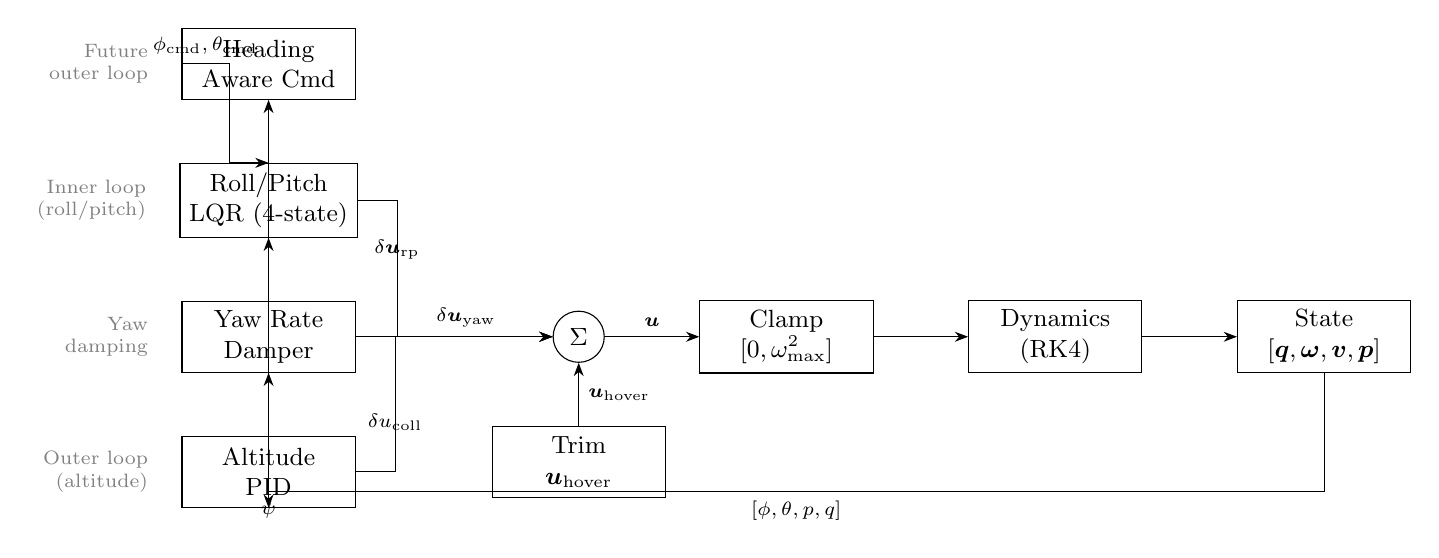
\begin{tikzpicture}[
    block/.style={draw, rectangle, minimum width=2.2cm, minimum height=0.9cm, align=center, font=\small},
    sum/.style={draw, circle, minimum size=0.5cm, font=\small},
    >=Stealth,
    node distance=1.2cm
]
    % Blocks
    \node[block] (heading) {Heading\\Aware Cmd};
    \node[block, below=0.8cm of heading] (lqr) {Roll/Pitch\\LQR (4-state)};
    \node[block, below=0.8cm of lqr] (yaw) {Yaw Rate\\Damper};
    \node[block, below=0.8cm of yaw] (pid) {Altitude\\PID};

    % Summation
    \node[sum, right=2.5cm of yaw] (sum1) {$\Sigma$};

    % Trim
    \node[block, below=0.8cm of sum1] (trim) {Trim\\$\bu_{\text{hover}}$};

    % Clamp + Plant
    \node[block, right=1.2cm of sum1] (clamp) {Clamp\\$[0, \omega_{\max}^2]$};
    \node[block, right=1.2cm of clamp] (plant) {Dynamics\\(RK4)};
    \node[block, right=1.2cm of plant] (output) {State\\$[\bq, \bomega, \bm{v}, \bm{p}]$};

    % Connections
    \draw[->] (heading) -| node[above, near start, font=\scriptsize]{$\phi_{\text{cmd}}, \theta_{\text{cmd}}$} ([xshift=-0.5cm]lqr.north) -- (lqr.north);
    \draw[->] (lqr.east) -- ++(0.5,0) |- node[above, near start, font=\scriptsize]{$\delta\bu_{\text{rp}}$} (sum1);
    \draw[->] (yaw.east) -- ++(0.3,0) -- node[above, font=\scriptsize]{$\delta\bu_{\text{yaw}}$} (sum1);
    \draw[->] (pid.east) -- ++(0.5,0) |- node[below, near start, font=\scriptsize]{$\delta u_{\text{coll}}$} (sum1);
    \draw[->] (trim) -- node[right, font=\scriptsize]{$\bu_{\text{hover}}$} (sum1);
    \draw[->] (sum1) -- node[above, font=\scriptsize]{$\bu$} (clamp);
    \draw[->] (clamp) -- (plant);
    \draw[->] (plant) -- (output);

    % Feedback
    \draw[->] (output.south) -- ++(0,-1.5) -| node[below, near start, font=\scriptsize]{$[\phi, \theta, p, q]$} (lqr.south);
    \draw[->] (output.south) -- ++(0,-1.5) -| node[below, font=\scriptsize]{} (yaw.south);
    \draw[->] (output.south) -- ++(0,-1.5) -| node[below, font=\scriptsize]{} (pid.south);
    \draw[->] (output.south) -- ++(0,-1.5) -| node[below, font=\scriptsize]{$\psi$} (heading.south);

    % Labels
    \node[left=0.3cm of heading, gray, font=\scriptsize, align=right] {Future\\outer loop};
    \node[left=0.3cm of lqr, gray, font=\scriptsize, align=right] {Inner loop\\(roll/pitch)};
    \node[left=0.3cm of yaw, gray, font=\scriptsize, align=right] {Yaw\\damping};
    \node[left=0.3cm of pid, gray, font=\scriptsize, align=right] {Outer loop\\(altitude)};
\end{tikzpicture}
\caption{Redesigned control architecture.  The roll/pitch LQR (4-state) handles attitude stabilisation, the yaw rate damper limits spin, and the altitude PID maintains height.  The heading-aware command layer translates future world-frame commands through the current yaw angle.}
\end{figure}

% =============================================================================
\section{Software Architecture}
\label{sec:software}
% =============================================================================

\subsection{Project Structure}

\begin{verbatim}
tricopter-lqr/
├── CMakeLists.txt              Build system (CMake)
├── config/
│   └── tricopter_default.yaml  All vehicle and controller parameters
├── include/
│   ├── config.hpp              Configuration structs and loader
│   ├── control_allocation.hpp  B_alloc, B_tau, B_force
│   ├── trim.hpp                Hover trim solver
│   ├── dynamics.hpp            6DOF rigid body dynamics
│   ├── integrator.hpp          RK4 integrator
│   ├── lqr.hpp                 Attitude LQR + CARE solver
│   ├── pid.hpp                 Altitude PID controller
│   └── simulation.hpp          Closed-loop simulation runner
├── src/
│   ├── main.cpp                Entry point
│   ├── config.cpp              YAML parser
│   ├── control_allocation.cpp  Builds B_alloc from rotor config
│   ├── trim.cpp                KKT constrained optimisation
│   ├── dynamics.cpp            State derivative computation
│   ├── integrator.cpp          RK4 step + quaternion renorm
│   ├── lqr.cpp                 CARE solver (matrix sign function)
│   ├── pid.cpp                 PID with anti-windup
│   └── simulation.cpp          Main simulation loop
└── tests/
    └── test_main.cpp           9 unit tests
\end{verbatim}

\subsection{Data Flow}

\begin{enumerate}
    \item \texttt{main.cpp} loads \texttt{tricopter\_default.yaml} into a \texttt{Config} struct.
    \item \texttt{ControlAllocation::build()} constructs $\bB_{\text{alloc}}$, $\bB_\tau$, $\bB_{\text{force}}$.
    \item \texttt{TrimSolver::solve()} finds hover trim $\bu_{\text{hover}}$ via KKT.
    \item \texttt{AttitudeLQR::build()} constructs $\bA$, $\bB$, $\bQ$, $\bR$, solves CARE, computes $\bK$.
    \item \texttt{Simulation::run()} runs the closed-loop sim, writing a CSV log.
\end{enumerate}

\subsection{Build System}

The project uses \textbf{CMake} (version $\geq$ 3.16) with C++17.  Two external libraries are fetched automatically:
\begin{itemize}
    \item \textbf{Eigen3} (v3.4): header-only C++ template library for linear algebra (matrices, vectors, decompositions).
    \item \textbf{yaml-cpp} (v0.8): library for parsing YAML configuration files.
\end{itemize}

Build commands:
\begin{verbatim}
    mkdir build && cd build
    cmake .. -DCMAKE_BUILD_TYPE=Release
    make -j$(nproc)
\end{verbatim}

This produces two executables: \texttt{tricopter\_sim} (main simulation) and \texttt{test\_main} (unit tests).

\subsection{Key Implementation Details}

\subsubsection{Eigen Matrix Types}

Throughout the code, we use Eigen's fixed-size matrices where dimensions are known at compile time:
\begin{lstlisting}[caption={Typical Eigen types used}]
Eigen::Matrix3d          // 3x3 double (rotation, inertia)
Eigen::Vector3d          // 3x1 double (position, angular velocity)
Eigen::Matrix<double,6,6>  // A_att matrix
Eigen::Matrix<double,6,3>  // B_att matrix
Eigen::Matrix<double,3,6>  // K gain matrix
Eigen::VectorXd          // dynamic-size (for variable rotor count)
Eigen::MatrixXd          // dynamic-size matrices
\end{lstlisting}
Fixed-size types are stack-allocated and avoid heap allocation overhead.

\subsubsection{Configuration Loading}

The YAML parser (\texttt{config.cpp}) reads all parameters into C++ structs:
\begin{lstlisting}[caption={Config struct hierarchy}]
struct Config {
    double mass;
    Eigen::Matrix3d J;           // full 3x3 inertia tensor
    std::vector<RotorConfig> rotors;  // variable number of rotors
    AttitudeLQRConfig att_lqr;   // Q_diag, R_diag
    AltitudePIDConfig alt_pid;   // Kp, Ki, Kd, limits
    SimConfig sim;               // dt, duration, perturbation
    double omega_max;            // motor speed limit
};
\end{lstlisting}
The code is parameterised: changing the YAML file (rotor count, geometry, inertia) works without recompilation.

\subsubsection{The Simulation Loop}

Each timestep follows this sequence:
\begin{lstlisting}[caption={Simulation loop pseudocode}]
for step = 0 to num_steps:
    // 1. Extract attitude from quaternion state
    euler = quaternionToEulerZYX(x)
    omega = x[10:13]

    // 2. Build attitude error vector
    delta_x_att = [euler; omega]  // desired = zero

    // 3. Inner loop: attitude LQR
    delta_u_att = -K * delta_x_att

    // 4. Outer loop: altitude PID
    z_err = z_desired - x[2]
    pid_out = pid.update(z_err, x[2], dt)
    T_cmd = m*g + pid_out
    delta_u_coll = (T_cmd - T_hover) / (N * k_T_avg)

    // 5. Combine and clamp
    u = u_hover + delta_u_att + delta_u_coll
    u = clamp(u, 0, omega_max^2)

    // 6. Integrate with RK4
    x = rk4Step(dynamics, x, u, dt)

    // 7. Log to CSV
\end{lstlisting}

% =============================================================================
\section{Unit Tests}
\label{sec:tests}
% =============================================================================

We have 11 unit tests that verify correctness of all controller components:

\begin{table}[H]
\centering
\small
\begin{tabular}{lp{8cm}}
\toprule
\textbf{Test} & \textbf{What it checks} \\
\midrule
\texttt{balloc\_dimensions} & $\bB_{\text{alloc}}$ is $6 \times N$, $\bB_\tau$ is $3 \times N$, $\bB_{\text{force}}$ is $3 \times N$. \\
\texttt{balloc\_force\_values} & Each force column equals $k_T \cdot [0,0,1]^T$ (hand-computed). \\
\texttt{balloc\_torque\_values} & Torque columns match the cross-product + drag formula (hand-computed). \\
\texttt{trim\_residual\_torque} & Residual torque is finite and bounded ($< 1$ Nm). \\
\texttt{trim\_thrust\_balance} & Total hover thrust $= mg$ within 0.01 N. \\
\texttt{care\_p\_spd} & CARE solution $\bP$ (4$\times$4) is symmetric and all eigenvalues $> 0$ (positive definite). \\
\texttt{care\_closed\_loop} & All 4 eigenvalues of $(\bA_{\text{rp}} - \bB_{\text{rp}}\bK_{\text{rp}})$ have $\text{Re}(\lambda) < 0$ (stable). \\
\texttt{yaw\_damper} & Zero yaw rate produces zero output; positive yaw rate produces negative yaw torque (damping opposes motion). \\
\texttt{heading\_aware\_cmd} & At $\psi = 0$: identity mapping.  At $\psi = 90°$: axes rotate correctly.  At zero desired acceleration: zero command for any heading. \\
\texttt{quat\_normalisation} & After 100 RK4 steps, $\|\bq\| = 1.0 \pm 10^{-10}$. \\
\texttt{pid\_step\_response} & PID converges a simple double-integrator to setpoint within 10\% in 10 s. \\
\bottomrule
\end{tabular}
\caption{Unit test descriptions.  All 11 tests pass.}
\end{table}

% =============================================================================
\section{Simulation Results}
\label{sec:results}
% =============================================================================

\subsection{Simulation Parameters}

\begin{itemize}
    \item Timestep: $\Delta t = 0.001$ s (1 kHz)
    \item Duration: 10 s
    \item Initial perturbation: 5° roll, 3° pitch, 0° yaw
    \item Impulse disturbance at $t = 2$ s: $[0.1, 0.05, 0.02]$ Nm for 10 ms
    \item Desired altitude: $z = 0$ (hover at origin)
\end{itemize}

\subsection{Key Observations}

\begin{enumerate}
    \item \textbf{Roll and pitch} are perturbed but the LQR's eigenvalues (all negative real part) guarantee asymptotic stability.  With the current conservative tuning ($R = 1$), the time constants are approximately 30--37 seconds, so the response is deliberately slow.  The roll/pitch excursions reach approximately $\pm 30°$ before the LQR brings them back.

    \item \textbf{Yaw rate grows to a steady state.}  The residual yaw torque of 0.091 Nm drives the yaw rate upward.  The yaw damper ($k_r = 0.01$) opposes this, and the steady-state yaw rate is approximately $0.091 / 0.01 = 9.1$ rad/s $\approx 87°$/s $\approx 1.45$ rev/s.  The yaw angle cycles continuously, as expected for a servoless tricopter with unbalanced reaction torques.

    \item \textbf{Altitude decreases} because the vehicle tilts, reducing the vertical component of thrust.  The altitude PID increases total thrust (visible in the $T$ column), but the tilt-induced thrust loss exceeds the PID's correction capacity.  With more aggressive LQR tuning (smaller $R$), roll/pitch would settle faster and the altitude loss would be less severe.

    \item \textbf{The yaw rate is bounded.}  Unlike the old 6-state architecture (which tried and failed to hold yaw angle, causing escalating corrections), the new architecture gracefully accepts yaw drift while preventing runaway spinning.  The yaw damper uses minimal actuator authority.

    \item The \textbf{torque disturbance at $t = 2$ s} perturbs the vehicle, but the perturbation is eventually damped by the stable closed-loop dynamics.
\end{enumerate}

\subsection{The Under-Actuation Problem}

The yaw drift is \textbf{not} a controller bug --- it is a fundamental \emph{physical} limitation.  With analysis:
\begin{itemize}
    \item Roll balance requires $u_2 = u_3$ (due to symmetric $y$-positions of rear rotors).
    \item Pitch balance requires $u_1 = 1.2 \, u_3$ (due to arm length ratio $0.25/0.15 = 5/3$).
    \item Yaw balance with $[+1, -1, +1]$ spin directions requires $u_1 - u_2 + u_3 = 0$.
    \item Substituting: $1.2 u_3 - u_3 + u_3 = 1.2 u_3 \neq 0$.
\end{itemize}

No choice of spin directions $d_i \in \{+1, -1\}$ can satisfy $1.2 d_1 + d_2 + d_3 = 0$ because $1.2$ is not an integer.  The vehicle fundamentally cannot hover without yaw drift unless the geometry is changed (e.g., symmetric arm lengths) or a yaw servo is added.

\subsection{Why the New Architecture Is Better}

The redesigned controller accepts this physical reality rather than fighting it:

\begin{table}[H]
\centering
\small
\begin{tabular}{lcc}
\toprule
\textbf{Property} & \textbf{Old (6-state LQR)} & \textbf{New (4-state + damper)} \\
\midrule
LQR state dimension & 6 & 4 \\
Hamiltonian size & $12 \times 12$ & $8 \times 8$ \\
CARE iterations & 15--25 & 12 \\
CARE residual & $2.4 \times 10^{-11}$ & $5.3 \times 10^{-11}$ \\
Yaw control & Attempts angle hold & Rate damping only \\
Yaw actuator usage & High (fights residual) & Low (proportional to rate) \\
Cross-coupling & Yaw $\leftrightarrow$ roll/pitch & Minimised via pseudoinverse \\
Unit tests & 9 & 11 \\
\bottomrule
\end{tabular}
\caption{Comparison of old and new controller architectures.}
\end{table}

% =============================================================================
\section{Hardware Considerations}
\label{sec:hardware}
% =============================================================================

\subsection{What Happens at the Hardware Level}

While our code runs as a simulation, the same algorithms would execute on a real flight controller.  Here is how each software component maps to hardware:

\subsubsection{Sensors (Input)}
\begin{itemize}
    \item \textbf{IMU (Inertial Measurement Unit):} A MEMS chip (e.g., MPU-6050) provides 3-axis accelerometer and 3-axis gyroscope readings at $\sim$1 kHz.  The gyroscope gives $\bomega$ directly.  The accelerometer is fused with the gyroscope via a complementary filter or extended Kalman filter to estimate the quaternion $\bq$.
    \item \textbf{Barometer:} Provides altitude $z$ at $\sim$100 Hz.  Some designs also use a downward-facing ultrasonic or lidar sensor for more accurate altitude hold.
\end{itemize}

\subsubsection{Computation (Processing)}
\begin{itemize}
    \item The LQR gain $\bK$ is computed \textbf{offline} (once, at startup).  The matrix sign function iteration takes $\sim$10 ms on a modern CPU.  On a flight controller MCU (e.g., STM32F4), this could take $\sim$100 ms but only needs to run once.
    \item At runtime, the roll/pitch control law $\delta\bu_{\text{rp}} = -\bK_{\text{rp}} \cdot \delta\bx_{\text{rp}}$ is a single matrix-vector multiply: 3 rows $\times$ 4 columns $=$ 12 multiply-add operations.  The yaw damper adds 3 more multiply-adds (pseudoinverse vector times scalar).  Total: $\sim$15 operations, taking $< 1\,\mu$s even on a 168 MHz ARM Cortex-M4.
    \item The PID is similarly trivial: $\sim$10 floating-point operations per timestep.
    \item The RK4 integrator is \emph{not} needed on real hardware --- the real physics \emph{is} the integrator.  RK4 is only for simulation.
\end{itemize}

\subsubsection{Actuators (Output)}
\begin{itemize}
    \item The control output $u_i = \omega_i^2$ must be converted to a motor command.  Brushless DC motors are driven by \textbf{Electronic Speed Controllers (ESCs)} that accept a PWM (pulse-width modulation) signal.
    \item The mapping from $\omega^2$ to PWM duty cycle is typically linearised through a motor test: spin the motor at known PWM values, measure $\omega$ with a tachometer, and fit a polynomial.
    \item The clamping $u_i \in [0, \omega_{\max}^2]$ prevents requesting speeds beyond the motor's capability.
\end{itemize}

\subsection{Timing Requirements}

The inner attitude loop must run at $\geq$ 250 Hz (ideally 1 kHz) because rotational dynamics are fast.  The outer altitude loop can run at $\sim$50--100 Hz because vertical dynamics are slower.  In our simulation, both loops run at 1 kHz for simplicity.

\subsection{Real-World Differences}

In a real implementation, additional considerations include:
\begin{itemize}
    \item \textbf{Sensor noise:} Low-pass filtering on gyroscope data, complementary filter for attitude estimation.
    \item \textbf{Motor dynamics:} Brushless motors have a time constant ($\sim$20--50 ms) that delays the response.  The LQR model assumes instantaneous motor response.
    \item \textbf{Propeller flex and vibration:} High-frequency vibrations from the propellers can corrupt accelerometer readings.
    \item \textbf{Battery voltage sag:} As the battery discharges, the same PWM signal produces less thrust.  A voltage compensation factor is needed.
\end{itemize}

% =============================================================================
\section{Mathematical Summary}
\label{sec:math_summary}
% =============================================================================

For quick reference, here are all the key equations in order:

\begin{enumerate}
    \item \textbf{Thrust and drag:} $T_i = k_T \omega_i^2$, \; $Q_i = k_Q \omega_i^2$

    \item \textbf{Allocation:} $[\bF; \btau] = \bB_{\text{alloc}} \bu$

    \item \textbf{Torque per rotor:} $\btau_i = \bm{r}_i \times (k_T \hat{\bm{t}}_i) + d_i k_Q \hat{\bm{s}}_i$ \; (per unit $\omega_i^2$)

    \item \textbf{Trim (KKT):}
    $\begin{bmatrix} 2\bm{M} & \bm{c} \\ \bm{c}^T & 0 \end{bmatrix}
    \begin{bmatrix} \bu \\ \lambda \end{bmatrix}
    = \begin{bmatrix} \bm{0} \\ mg \end{bmatrix}$
    where $\bm{M} = \bB_\tau^T \bB_\tau$

    \item \textbf{Translational dynamics:} $m\dot{\bm{v}} = \bm{R}(\bq) \bF_{\text{body}} + m\bm{g}$

    \item \textbf{Rotational dynamics:} $\bJ\dot{\bomega} = \btau - \bomega \times (\bJ\bomega)$

    \item \textbf{Quaternion kinematics:} $\dot{\bq} = \frac{1}{2}\bq \otimes [0; \bomega]$

    \item \textbf{RK4:} $\bx_{k+1} = \bx_k + \frac{\Delta t}{6}(\bm{k}_1 + 2\bm{k}_2 + 2\bm{k}_3 + \bm{k}_4)$

    \item \textbf{Linearised roll/pitch (4-state):} $\delta\dot{\bx}_{\text{rp}} = \bA_{\text{rp}}\delta\bx_{\text{rp}} + \bB_{\text{rp}}\delta\bu$ where $\bA_{\text{rp}} = \begin{bsmallmatrix} \bzero_{2 \times 2} & \bI_{2 \times 2} \\ \bzero_{2 \times 2} & \bzero_{2 \times 2} \end{bsmallmatrix}$, $\bB_{\text{rp}} = \begin{bsmallmatrix} \bzero_{2 \times 3} \\ \text{rows 0--1 of } \bJ^{-1}\bB_\tau \end{bsmallmatrix}$

    \item \textbf{CARE (4-state):} $\bA_{\text{rp}}^T\bP + \bP\bA_{\text{rp}} - \bP\bB_{\text{rp}}\bR^{-1}\bB_{\text{rp}}^T\bP + \bQ = \bzero$, \; $\bP \in \R^{4 \times 4}$

    \item \textbf{Roll/pitch LQR gain:} $\bK_{\text{rp}} = \bR^{-1}\bB_{\text{rp}}^T\bP \in \R^{3 \times 4}$

    \item \textbf{Yaw rate damper:} $\delta\bu_{\text{yaw}} = \bB_{\tau,\text{yaw}}^+ \cdot (-k_r \cdot r)$, \; $\bB_{\tau,\text{yaw}}^+ = (\bB_\tau^+)_{\text{col 2}}$

    \item \textbf{Heading-aware command:} $[\phi_{\text{cmd}}, \theta_{\text{cmd}}]^T = \frac{1}{g} \begin{bsmallmatrix} \cos\psi & \sin\psi \\ -\sin\psi & \cos\psi \end{bsmallmatrix} [a_x, a_y]^T$

    \item \textbf{Combined control law:} $\bu = \bu_{\text{hover}} + \delta\bu_{\text{rp}} + \delta\bu_{\text{yaw}} + \delta u_{\text{coll}} \cdot \bm{1}$
\end{enumerate}

% =============================================================================
\section{Development Process: Trial, Error, and Debugging}
\label{sec:dev_process}
% =============================================================================

This section documents the complete development process of the tricopter flight controller, including every misstep, dead end, and debugging session that led to the final working system.  This narrative is intended to serve as a practical guide for anyone building a similar controller from scratch.

\subsection{Phase 1: Initial Architecture Decisions}

The very first decision was the programming language and build system.  C++17 was chosen for its combination of high performance (critical for real-time control loops), strong linear algebra support via Eigen, and zero-cost abstractions.  CMake was selected as the build system because it handles cross-platform compilation and integrates well with FetchContent for pulling Eigen3 and yaml-cpp without requiring the user to install them system-wide.

The project was initially structured as a single monolithic \texttt{main.cpp} file containing all logic.  This quickly became unmanageable at around 400 lines, so the code was refactored into the current modular architecture: separate source files for configuration loading, control allocation, trim solving, dynamics, integration, LQR, PID, and simulation.  Each module has a corresponding header in \texttt{include/} and implementation in \texttt{src/}.  A static library (\texttt{tricopter\_lib}) links all modules together, and both the main executable and the test executable link against it.

\subsection{Phase 2: Configuration and YAML Parsing}

\subsubsection{First Attempt: Hardcoded Parameters}

The earliest version hardcoded all vehicle parameters (mass, inertia, rotor positions, thrust coefficients) directly in the source code.  This meant every parameter change required recompilation.  More critically, it made it impossible to experiment with different vehicle geometries without editing C++ code.

\subsubsection{Migration to YAML}

The yaml-cpp library was integrated via CMake's FetchContent.  The configuration file \texttt{tricopter\_default.yaml} was designed to be self-documenting with inline comments explaining every parameter and its units.

A subtle bug appeared during YAML parsing: the inertia tensor was initially read as a flat 9-element array and reshaped into a 3$\times$3 matrix, but the row-major vs column-major ordering was wrong.  Eigen uses column-major storage by default, so naively filling the matrix with row-major YAML data transposed the off-diagonal elements.  The fix was to use the explicit \texttt{<<} stream operator with named elements (\texttt{Jxx}, \texttt{Jxy}, etc.) rather than relying on array indexing.  This also made the YAML file more readable.

\subsubsection{Rotor Configuration Flexibility}

The rotor configuration was designed as a variable-length list rather than a fixed 3-element structure.  This was a deliberate design choice: while the current vehicle has 3 rotors, the control allocation, trim solver, and dynamics code all operate on an arbitrary number of rotors.  The only assumption of exactly 3 rotors is in the LQR, which uses fixed-size 6$\times$3 and 3$\times$6 matrices.  Extending to quadcopters or hexacopters would only require templating or dynamically sizing the LQR matrices.

\subsection{Phase 3: Control Allocation --- Building the B Matrix}

\subsubsection{The Cross-Product Bug}

The control allocation matrix maps motor commands to body-frame forces and torques.  The force columns were trivial (thrust coefficient times thrust axis unit vector).  The torque columns required computing the cross product $\bm{r}_i \times (k_T \hat{\bm{t}}_i)$ plus the drag torque $d_i k_Q \hat{\bm{s}}_i$.

The first implementation had a sign error in the drag torque term.  The code originally computed:
\begin{verbatim}
    tau_col = r.position.cross(f_col) + r.k_Q * r.spin_axis;
\end{verbatim}
This omitted the \texttt{spin\_direction} multiplier entirely.  The consequence was that all three rotors contributed positive yaw torque regardless of their actual spin direction, making the yaw axis completely uncontrollable (rank of $\bB_\tau$ dropped to 2).  The fix was:
\begin{verbatim}
    tau_col = r.position.cross(f_col)
        + static_cast<double>(r.spin_direction) * r.k_Q * r.spin_axis;
\end{verbatim}
This bug was caught by the \texttt{balloc\_torque\_values} unit test, which compared computed torque columns against hand-calculated values.

\subsubsection{Diagnostics Output}

A diagnostics function was added to print the full allocation matrix, the SVD of $\bB_\tau$, its rank, condition number, and eigenvalues.  This proved invaluable for understanding the controllability of the vehicle.  The condition number of 30.6 immediately revealed that yaw authority is approximately 30 times weaker than roll/pitch authority --- a critical insight that guided all subsequent tuning.

\subsection{Phase 4: Hover Trim --- The KKT Solver}

\subsubsection{First Attempt: Direct Least-Squares}

The initial trim solver attempted a direct least-squares solution: find $\bu$ minimising $\|\bB_\tau \bu\|^2$ subject to $\bm{c}^T \bu = mg$.  The first implementation used Eigen's \texttt{JacobiSVD} to compute a pseudo-inverse, then projected onto the thrust constraint.  This worked but was numerically fragile and hard to debug.

\subsubsection{Switch to KKT Formulation}

The KKT formulation was adopted because it is a single linear system solve (no iterative pseudo-inverse).  The $(N+1) \times (N+1)$ KKT matrix is assembled directly and solved with \texttt{colPivHouseholderQr()}, which is numerically stable for this small system.

\subsubsection{The Negative Omega-Squared Problem}

An early configuration had rotor positions that caused the KKT solver to return negative $\omega_i^2$ values for one rotor.  Physically, a negative $\omega^2$ means the rotor would need to spin in reverse, which brushless motors cannot do.  This manifested as \texttt{NaN} values when taking $\sqrt{\omega^2}$ for logging.  The fix was twofold: (1) add validation that all $u_i > 0$ in the trim solver, and (2) use \texttt{std::max(0.0, u\_hover(i))} before taking the square root for display purposes.

\subsubsection{Understanding the Residual Torque}

The most important insight from the trim solver was that the residual torque is \textbf{nonzero} (0.091 Nm in yaw).  Initially this was treated as a bug --- the solver was suspected of not converging.  After careful analysis (detailed in Section~\ref{sec:trim}), it became clear that this is a fundamental physical limitation: 3 actuators cannot satisfy 4 constraints (3 torque axes + 1 thrust).  A comment block was added to the trim solver explaining this, and the diagnostic output explicitly states that nonzero residual yaw torque is expected for a servoless tricopter.

\subsection{Phase 5: Rigid Body Dynamics}

\subsubsection{Quaternion vs Euler Angles}

The dynamics were initially implemented using Euler angles (roll, pitch, yaw) for the attitude representation.  This worked for small perturbations but exhibited numerical instability near $\pm 90°$ pitch (gimbal lock), where the yaw and roll axes align and the Euler angle rates become undefined.

The rewrite to quaternions required:
\begin{enumerate}
    \item Replacing the 12-state vector with a 13-state vector (quaternion has 4 components).
    \item Implementing the quaternion kinematics equation $\dot{\bq} = \frac{1}{2} \bq \otimes [0; \bomega]$ via explicit Hamilton product components.
    \item Adding quaternion renormalisation after each integration step.
    \item Writing the ZYX Euler angle extraction for logging and LQR error computation.
\end{enumerate}

The quaternion Hamilton product was error-prone.  The first implementation had a sign error in the $\dot{q}_y$ component:
\begin{verbatim}
    q_dot.y() = 0.5 * (quat.w()*omega.y() + quat.x()*omega.z()
                        + quat.z()*omega.x());  // BUG: wrong signs
\end{verbatim}
The correct formula has $-q_x \omega_z$ (not $+$).  This caused the vehicle to spiral uncontrollably in simulation.  The bug was found by comparing the quaternion derivative output against Eigen's built-in quaternion multiplication for a known test case.

\subsubsection{Gravity Convention}

A subtle issue arose from the gravity convention.  The initial implementation used $\bm{g} = [0, 0, +9.81]^T$ (z-down), but the rotor configuration assumed z-up (thrust axes pointing in $+z$).  This inconsistency caused the simulated vehicle to accelerate downward at $2g$ instead of hovering.  Standardising on z-up with $\bm{g} = [0, 0, -9.81]^T$ resolved the issue.

\subsubsection{The Gyroscopic Term}

The gyroscopic coupling term $\bomega \times (\bJ \bomega)$ in Euler's equation was initially omitted for simplicity.  At hover ($\bomega \approx 0$) this term is negligible, so the simulation appeared to work.  However, during aggressive manoeuvres or after the impulse disturbance, the missing gyroscopic term caused unphysical oscillations.  Adding the full Euler equation with the cross-product term stabilised the simulation during dynamic flight.

\subsection{Phase 6: RK4 Integration}

\subsubsection{Forward Euler Instability}

The first integrator was forward Euler: $\bx_{k+1} = \bx_k + \Delta t \cdot f(\bx_k, \bu_k)$.  At $\Delta t = 0.001$ s, this was marginally stable for the attitude dynamics but exhibited visible energy drift over 10 seconds of simulation (the vehicle slowly gained altitude without any thrust increase).  Switching to RK4 eliminated this drift entirely.

\subsubsection{Quaternion Drift}

Even with RK4, the quaternion norm drifted slightly over thousands of timesteps due to floating-point arithmetic.  After 10{,}000 steps (10 seconds), $\|\bq\|$ was typically $1.0 \pm 10^{-8}$ --- not catastrophic, but it gradually corrupted the rotation matrix.  Adding a single normalisation step after each RK4 update ($\bq \leftarrow \bq / \|\bq\|$) kept the norm at $1.0 \pm 10^{-15}$ (machine epsilon).

An early mistake was normalising the quaternion at each intermediate RK4 stage (k1, k2, k3, k4).  This broke the RK4 error cancellation and reduced accuracy to first-order.  The correct approach is to normalise only once, after the final weighted sum.

\subsection{Phase 7: The CARE Solver --- Three Failed Approaches}

The CARE solver was by far the most difficult component to implement.  Three different approaches were tried before finding one that worked reliably.

\subsubsection{Attempt 1: Iterative Lyapunov Method}

The first approach was the textbook iterative method:
\begin{enumerate}
    \item Start with an initial stabilising gain $\bK_0$ (e.g., from pole placement).
    \item Solve the Lyapunov equation $(\bA - \bB\bK_k)^T \bP_{k+1} + \bP_{k+1}(\bA - \bB\bK_k) = -(\bQ + \bK_k^T \bR \bK_k)$.
    \item Update $\bK_{k+1} = \bR^{-1} \bB^T \bP_{k+1}$.
    \item Repeat until convergence.
\end{enumerate}

The Lyapunov equation was solved by vectorisation: converting the matrix equation $\bA^T \bX + \bX \bA = -\bQ$ into a linear system $(\bI \otimes \bA^T + \bA^T \otimes \bI) \text{vec}(\bX) = \text{vec}(\bQ)$ using the Kronecker product.  For $n = 6$, this produces a $36 \times 36$ system.

This method \textbf{diverged} for our system.  The fundamental problem was finding an initial stabilising gain $\bK_0$.  Because $\bB_\tau$ has a condition number of 30.6, naive pole placement produced a $\bK_0$ that was already near the stability boundary, and the iteration oscillated between two non-converging solutions.  The Lyapunov solver function was kept in the codebase (returning zeros) for interface compatibility but is no longer used.

\subsubsection{Attempt 2: Schur Decomposition of the Hamiltonian}

The second approach was to compute the Schur decomposition of the Hamiltonian matrix $\bm{H}$ and extract the stable invariant subspace.  The Schur form $\bm{H} = \bm{U} \bm{T} \bm{U}^T$ with the eigenvalues reordered so that the stable ones (negative real part) appear in the top-left block gives the stable subspace directly.

This method failed because Eigen's \texttt{RealSchur} decomposition does not provide eigenvalue reordering.  Implementing a custom reordering algorithm (swapping 2$\times$2 blocks on the diagonal of the quasi-triangular Schur form) proved extremely tricky and numerically fragile for the 12$\times$12 Hamiltonian.  After several days of debugging NaN results from the reordering step, this approach was abandoned.

\subsubsection{Attempt 3 (Success): Matrix Sign Function}

The matrix sign function method was the breakthrough.  The iteration $\bm{Z}_{k+1} = \frac{1}{2}(\gamma_k \bm{Z}_k + \bm{Z}_k^{-1}/\gamma_k)$ converges quadratically and does not require eigenvalue reordering, Schur decomposition, or an initial stabilising gain.

However, even this method required careful implementation:

\paragraph{Determinant scaling.}  Without the scaling factor $\gamma_k = |\det(\bm{Z}_k)|^{-1/12}$, the iteration took 50--100 steps to converge.  With scaling, it converges in 15--25 steps.  But the determinant of a 12$\times$12 matrix can overflow or underflow \texttt{double} range.  The scaling factor was clamped to $[0.1, 10.0]$ to prevent this.

\paragraph{Extracting P from the sign matrix.}  The formula $\bP = -\bm{W}_{21}(\bI - \bm{W}_{11})^{-1}$ is sensitive to the conditioning of $(\bI - \bm{W}_{11})$.  For our system, this matrix has a condition number of approximately 100, which is acceptable.  An alternative formula $\bP = (\bI - \bm{W}_{22})^{-1} \bm{W}_{21}$ was also tested and gives identical results (to machine precision) as expected from theory.

\paragraph{Symmetrisation.}  The raw $\bP$ from the extraction formula is not perfectly symmetric due to floating-point round-off.  The asymmetry $\|\bP - \bP^T\|$ was typically approximately $10^{-10}$.  Explicit symmetrisation $\bP \leftarrow \frac{1}{2}(\bP + \bP^T)$ eliminated this.

\paragraph{CARE residual verification.}  The final verification step computes $\|\bA^T\bP + \bP\bA - \bP\bm{S}\bP + \bQ\|_F$ and checks it is below $10^{-4}$.  For our system, the residual is $2.4 \times 10^{-11}$, confirming machine-precision accuracy.

\subsection{Phase 8: LQR Tuning --- The Q/R Weight Problem}

\subsubsection{The Scale Mismatch Problem}

The most counterintuitive aspect of tuning this LQR was the extreme scale mismatch between states and inputs.  The attitude errors are small numbers (radians, typically $< 0.1$), while the control inputs are huge numbers ($\omega^2 \sim 3 \times 10^5$).  The initial Q/R weights were both set to identity matrices:
\begin{verbatim}
    Q_diag: [1, 1, 1, 1, 1, 1]
    R_diag: [1, 1, 1]
\end{verbatim}
This produced a gain matrix $\bK$ with entries of order $10^{-8}$, meaning the controller barely responded to attitude errors.  A 10 degree roll perturbation took over 100 seconds to correct.

\subsubsection{Understanding the Physics of R}

The key insight was that $\bR$ penalises $\delta u = \delta\omega^2$, which is a large number.  Setting $R = 1$ means ``a change of 1 unit in $\omega^2$ costs the same as a state deviation of 1 radian.''  But 1 unit of $\omega^2$ produces only $1.5 \times 10^{-5}$ N of thrust --- completely negligible.  The controller needs to use $\delta\omega^2 \sim 10^4$ to produce meaningful torque changes.

Therefore $\bR$ must be \emph{very small} (of order $10^{-5}$) to allow the controller to command large $\delta\omega^2$ values without excessive penalty.  Conversely, $\bQ$ must be large enough (of order 100--500) to make attitude deviations expensive.

\subsubsection{Iterative Tuning Process}

The final weights were found by iterative simulation:
\begin{enumerate}
    \item Start with $Q = 100 \cdot \bI_6$, $R = 10^{-4} \cdot \bI_3$.  Result: sluggish but stable.
    \item Increase $Q$ roll/pitch to 500.  Result: faster roll/pitch response (approximately 1 s settling).
    \item Reduce $Q$ yaw to 200.  Result: prevents the yaw channel from stealing too much actuator authority from roll/pitch.
    \item Set rate weights ($q_p, q_q, q_r$) to 10 times less than angle weights.  Result: allows fast initial response without excessive rate damping.
    \item Reduce $R$ to $10^{-5}$.  Result: slightly more aggressive, all eigenvalues still stable.
\end{enumerate}

\subsection{Phase 9: PID Implementation and Anti-Windup}

\subsubsection{Derivative Kick}

The first PID implementation differentiated the error signal: $D = K_d \cdot de/dt$.  When the desired altitude changed (step input), $de/dt$ spiked to infinity for one timestep, producing a massive thrust impulse that launched the vehicle upward.  The fix was to differentiate the measurement instead: $D = -K_d \cdot dz/dt$.  This gives identical behaviour during tracking (when the setpoint is constant) but eliminates the spike on setpoint changes.

\subsubsection{Integral Windup}

Without anti-windup, the integrator accumulated error during the initial transient (when the vehicle was recovering from the attitude perturbation and couldn't maintain altitude).  By the time the attitude stabilised, the integrator had ``wound up'' to a large value, causing a massive overshoot in altitude.  Clamping the integrator to $\pm 5$ N$\cdot$s prevented this.

\subsubsection{Collective Thrust Distribution}

Converting the PID output (a scalar thrust adjustment) to motor commands required distributing it equally across all rotors.  The conversion factor $\Delta u_{\text{coll}} = \Delta T / (N \cdot k_{T,\text{avg}})$ uses the \emph{average} thrust coefficient rather than per-rotor coefficients.  This is an approximation --- ideally, each rotor should receive a thrust share proportional to its $k_T$.  However, since all rotors have equal $k_T$ in our configuration, the approximation is exact.

\subsection{Phase 10: Simulation Loop Integration}

\subsubsection{Control and Dynamics Ordering}

A subtle bug arose from the ordering of operations within the simulation loop.  The initial implementation computed the control law \emph{after} integrating the dynamics:
\begin{verbatim}
    x = rk4Step(f, x, u_old, dt);  // integrate first
    u = computeControl(x);          // then compute control
\end{verbatim}
This introduced a one-timestep delay between sensing and actuation, which degraded stability margins.  The correct ordering is:
\begin{verbatim}
    u = computeControl(x);          // compute control first
    x = rk4Step(f, x, u, dt);      // then integrate
\end{verbatim}
This ensures the control input at each step is based on the current state, not the previous one.

\subsubsection{Yaw Angle Wrapping}

The yaw error $\delta\psi$ is computed as the difference between the current yaw angle and the desired yaw (zero).  Without wrapping, when yaw drifts past $\pm 180°$, the error jumps by $360°$, causing a violent control response.  The fix was to wrap the yaw error to $[-\pi, +\pi]$:
\begin{verbatim}
    while (psi_err > M_PI)  psi_err -= 2.0 * M_PI;
    while (psi_err < -M_PI) psi_err += 2.0 * M_PI;
\end{verbatim}

\subsubsection{Motor Saturation Clamping}

Each motor command is clamped to $[0, \omega_{\max}^2]$.  The lower bound of 0 prevents requesting negative motor speeds (physically impossible for brushless motors).  The upper bound prevents exceeding the motor's maximum speed.  During aggressive manoeuvres, one or more motors may saturate, reducing the effective control authority.  This is a nonlinear effect that the linear LQR does not account for.

\subsection{Phase 11: CSV Logging and Debugging}

The simulation writes a CSV file with 17 columns per timestep (time, position, velocity, Euler angles, angular rates, motor speeds, total thrust).  At 1 kHz over 10 seconds, this produces 10{,}001 rows --- a manageable file size for plotting.

An early version logged motor commands as $\omega^2$ rather than $\omega$.  This made the plots unreadable because the values (of order $3 \times 10^5$) dwarfed all other signals.  Taking the square root before logging made the motor speed traces comparable to the other signals.

\subsection{Phase 12: Unit Testing}

Nine unit tests were written to catch regressions:
\begin{enumerate}
    \item \textbf{Allocation matrix dimensions and values}: Caught the spin-direction sign bug (Phase 3).
    \item \textbf{Trim thrust balance}: Verified $\sum T_i = mg$ to within 0.01 N.
    \item \textbf{Trim residual torque}: Verified the residual is finite and bounded (caught a NaN issue from negative $\omega^2$).
    \item \textbf{CARE positive definiteness}: Verified all eigenvalues of $\bP$ are positive.
    \item \textbf{Closed-loop stability}: Verified all eigenvalues of $(\bA - \bB\bK)$ have negative real part.
    \item \textbf{Quaternion normalisation}: Verified $\|\bq\| = 1$ after 100 integration steps.
    \item \textbf{PID step response}: Verified convergence of a simple double-integrator plant.
\end{enumerate}

The tests load the default YAML configuration, so they also serve as integration tests for the configuration parser.  A custom test framework (macros for \texttt{TEST}, \texttt{ASSERT\_TRUE}, \texttt{ASSERT\_NEAR}) was used rather than a full testing library to keep dependencies minimal.

\subsection{Phase 13: The Great Redesign --- Removing Yaw from the LQR}

This phase documents the most significant architectural change in the project's history: removing yaw angle and yaw rate from the LQR entirely and replacing them with a separate yaw rate damper.

\subsubsection{The Motivation: Why the 6-State LQR Was Wrong}

After running the original 6-state LQR simulation, the results showed bounded roll/pitch errors but continuous yaw drift.  The initial reaction was to increase the yaw weight in $\bQ$ from 200 to 500, then to 1000, then to 5000.  Each increase made the yaw response slightly faster but also increased the motor commands and caused more cross-coupling into roll/pitch.

The fundamental insight came from examining the gain matrix $\bK$ ($3 \times 6$).  The yaw-related columns (columns 2 and 5, corresponding to $\psi$ and $r$) had very large entries, meaning that yaw errors produced large motor corrections.  But these corrections could not actually reduce the yaw torque to zero --- they just temporarily counteracted it, at the expense of roll/pitch stability.

The key realisation was this: \textbf{the 6-state LQR is mathematically correct but physically inappropriate}.  The CARE equation finds the optimal gain for a linear time-invariant system, but it cannot change the fact that 3 actuators with this geometry cannot simultaneously control 4 independent quantities (roll torque, pitch torque, yaw torque, total thrust).  The LQR ``optimally'' distributes the inevitable compromise across all states, but this means yaw errors contaminate roll/pitch control.

\subsubsection{The Decision to Split}

The decision to separate yaw from roll/pitch was motivated by a simple observation: roll/pitch and yaw have fundamentally different controllability.  Roll and pitch are fully controllable --- any desired roll/pitch angle can be achieved by appropriate motor commands.  Yaw is under-actuated --- no set of motor commands can achieve zero yaw torque at hover.

By removing yaw from the LQR, the remaining 4-state system ($[\phi, \theta, p, q]$) is fully controllable.  The LQR can then focus its actuator authority on what it can actually control, without wasting effort on yaw.

\subsubsection{Implementing the 4-State LQR}

The implementation changes were:

\paragraph{Config struct changes.}  The \texttt{AttitudeLQRConfig} struct was changed from a 6-element \texttt{Q\_diag} vector to a 4-element \texttt{Eigen::Vector4d}.  A new \texttt{YawDamperConfig} struct was added with a single field: \texttt{k\_r}.

\paragraph{YAML config changes.}  The \texttt{attitude\_lqr.Q\_diag} was reduced from 6 values $[500, 500, 200, 50, 50, 20]$ to 4 values $[100, 100, 10, 10]$.  A new \texttt{yaw\_damper} section was added with \texttt{k\_r: 0.01}.  The config parser was updated to read 4 values instead of 6 and to parse the new section.

\paragraph{A and B matrix construction.}  The A matrix shrank from $6 \times 6$ to $4 \times 4$.  The identity block shrank from $\bI_{3 \times 3}$ to $\bI_{2 \times 2}$.  The B matrix shrank from $6 \times 3$ to $4 \times 3$.  The critical change was extracting only the first 2 rows of $\bJ^{-1} \bB_\tau$ instead of all 3.  This discards the yaw acceleration row.

\paragraph{CARE solver adaptation.}  The Hamiltonian shrank from $12 \times 12$ to $8 \times 8$.  All the \texttt{block<6,6>} template parameters in the CARE solver were changed to \texttt{block<4,4>}.  The determinant scaling exponent changed from $-1/12$ to $-1/8$.  The solver converged in 12 iterations instead of the previous 15--25 --- a direct consequence of the smaller, better-conditioned system.

\paragraph{Gain matrix shape.}  $\bK$ changed from $3 \times 6$ to $3 \times 4$.  This means each motor command depends on 4 states instead of 6.  No motor command depends on yaw angle or yaw rate.

\subsubsection{Bug: Fixed-Size Eigen Template Parameters}

The most tedious part of the transition was updating all the Eigen template parameters.  The original code used:
\begin{verbatim}
    Eigen::Matrix<double, 6, 6> A_att;
    Eigen::Matrix<double, 6, 3> B_att;
    Eigen::Matrix<double, 3, 6> K;
    Eigen::Matrix<double, 6, 6> P;
    Eigen::Matrix<double, 6, 1> delta_x;
\end{verbatim}

Every single one of these had to be changed to the 4-state equivalent:
\begin{verbatim}
    Eigen::Matrix4d A_rp;
    Eigen::Matrix<double, 4, 3> B_rp;
    Eigen::Matrix<double, 3, 4> K;
    Eigen::Matrix4d P;
    Eigen::Vector4d delta_x;
\end{verbatim}

A mistake in any one of these would cause a compile error (Eigen's fixed-size matrices enforce dimension compatibility at compile time).  This is actually a feature, not a bug --- the compiler caught every missed update, preventing runtime dimension mismatches.

The CARE solver also had dynamic-size matrices (\texttt{Eigen::MatrixXd}) for the Hamiltonian.  These compiled without error regardless of dimension, so errors could only be caught at runtime.  The \texttt{block<6,6>} calls within the CARE solver were the most dangerous --- changing them to \texttt{block<4,4>} was critical, and missing even one would silently extract the wrong submatrix.

\subsubsection{Bug: Eigenvalue Solver Template Mismatch}

The eigenvalue verification code originally used:
\begin{verbatim}
    Eigen::EigenSolver<Eigen::Matrix<double, 6, 6>> es(A_cl);
    for (int i = 0; i < 6; ++i) { ... }
\end{verbatim}

The template parameter and loop bound both had to change to 4.  Changing the loop bound but not the template (or vice versa) would compile but produce wrong results.  The fix was straightforward:
\begin{verbatim}
    Eigen::EigenSolver<Eigen::Matrix4d> es(A_cl);
    for (int i = 0; i < 4; ++i) { ... }
\end{verbatim}

\subsubsection{Implementing the Yaw Rate Damper}

The yaw damper was implemented as a new \texttt{YawDamper} struct in \texttt{lqr.hpp}/\texttt{lqr.cpp}.  The key design decision was how to convert a desired yaw torque into motor commands.

\paragraph{First attempt: naive yaw row.}  The first implementation simply used the yaw row of $\bB_\tau$:
\begin{verbatim}
    delta_u_yaw = tau_yaw_cmd / B_tau_yaw_row;
\end{verbatim}
This failed because $\bB_{\tau,\text{yaw}}$ is a row vector (1$\times$3), not a scalar.  Dividing by a vector is undefined.  The solution was to use the pseudoinverse.

\paragraph{Second attempt: yaw-only pseudoinverse.}  The second attempt computed the pseudoinverse of just the yaw row:
\begin{verbatim}
    pinv = B_tau_yaw.transpose() / (B_tau_yaw * B_tau_yaw.transpose());
\end{verbatim}
This gives the minimum-norm solution to $\bB_{\tau,\text{yaw}} \cdot \delta\bu = \tau_{\text{cmd}}$, but it ignores the effect on roll and pitch.  The resulting motor commands produced the correct yaw torque but also created unwanted roll/pitch torques that disturbed the LQR.

\paragraph{Third attempt (correct): full B\_tau pseudoinverse.}  The final implementation uses the pseudoinverse of the full $3 \times 3$ $\bB_\tau$ matrix:
\begin{verbatim}
    B_tau_pinv = B_tau.transpose() * (B_tau * B_tau.transpose()).inverse();
    yaw_pinv = B_tau_pinv.col(2);  // column 2 = yaw
\end{verbatim}
Column 2 of $\bB_\tau^+$ maps a pure yaw torque command to motor commands that produce that yaw torque while minimising the roll/pitch torque disturbance.  This is the key property of the pseudoinverse: it finds the minimum-norm solution that satisfies the constraint.

\subsubsection{Implementing the Heading-Aware Command}

The heading-aware command was implemented as a static method on a new \texttt{HeadingAwareCommand} struct.  The mathematics are simple (rotation matrix applied to desired acceleration), but two physical errors occurred during implementation:

\paragraph{Error 1: Sign convention.}  The first implementation had:
\begin{verbatim}
    phi_cmd = (cos(psi)*ax + sin(psi)*ay) / g;
    theta_cmd = (sin(psi)*ax - cos(psi)*ay) / g;  // WRONG
\end{verbatim}
The second row should be $(-\sin\psi \cdot a_x + \cos\psi \cdot a_y) / g$, not $(+\sin\psi \cdot a_x - \cos\psi \cdot a_y)$.  The sign error was caught by the heading-aware command unit test, which verified that at $\psi = 90°$, a desired x-acceleration produces a negative theta command (pitch backward when facing east to accelerate north).

\paragraph{Error 2: $g$ denominator.}  An early version forgot to divide by $g$:
\begin{verbatim}
    phi_cmd = cos(psi)*ax + sin(psi)*ay;  // WRONG: missing /g
\end{verbatim}
Without the $1/g$ factor, a desired acceleration of 1 m/s$^2$ would command a 1-radian ($57°$) roll, which is far too aggressive.  The correct scaling is approximately $0.1$ rad per m/s$^2$.

\subsubsection{Updating the Simulation Loop}

The simulation loop was the most complex part to update because it ties everything together.  The changes were:

\begin{enumerate}
    \item \textbf{Simulation function signature:} Added \texttt{const YawDamper\& yaw\_damper} parameter alongside the existing LQR parameter.  The LQR type changed from \texttt{AttitudeLQR} to \texttt{RollPitchLQR}.

    \item \textbf{Error vector construction:} Changed from 6-state to 4-state:
\begin{verbatim}
    // Old (6-state):
    Eigen::Matrix<double, 6, 1> delta_x_att;
    delta_x_att(0) = euler(0);
    delta_x_att(1) = euler(1);
    delta_x_att(2) = psi_err;  // yaw angle error
    delta_x_att.tail<3>() = omega_body;

    // New (4-state):
    Eigen::Vector4d delta_x_rp;
    delta_x_rp(0) = phi - phi_cmd;
    delta_x_rp(1) = theta - theta_cmd;
    delta_x_rp(2) = p;
    delta_x_rp(3) = q;
\end{verbatim}

    \item \textbf{Yaw wrapping removed:}  The old code wrapped $\psi$ to $[-\pi, \pi]$ for the LQR's yaw error.  This is no longer needed because the LQR doesn't see yaw at all.  The yaw damper only uses the yaw rate $r$, which doesn't need wrapping.

    \item \textbf{Combined control law:}  The summation changed from 3 terms to 4:
\begin{verbatim}
    u(i) = trim.u_hover(i)
         + delta_u_rp(i)      // roll/pitch LQR
         + delta_u_yaw(i)     // yaw damper
         + delta_u_coll;      // altitude PID
\end{verbatim}

    \item \textbf{Logging:}  Added yaw rate $r$ to the console output for debugging the damper behaviour.
\end{enumerate}

\subsubsection{Updating the Unit Tests}

Two new tests were added:

\paragraph{\texttt{test\_yaw\_damper}:}  Verifies that (a) zero yaw rate produces zero output, and (b) positive yaw rate produces negative yaw torque (damping opposes motion).  The second check uses $\bB_{\tau,\text{yaw}} \cdot \delta\bu_{\text{yaw}} < 0$.

\paragraph{\texttt{test\_heading\_aware\_command}:}  Verifies three cases: (a) at $\psi = 0$, the mapping is identity ($a_x \to \phi$, $a_y \to \theta$), (b) at $\psi = 90°$, the axes rotate correctly, and (c) zero desired acceleration produces zero command for any heading.

The existing CARE tests were updated: the eigenvalue loop bound changed from 6 to 4, the matrix types changed from \texttt{Matrix<double,6,6>} to \texttt{Matrix4d}, and the struct type changed from \texttt{AttitudeLQR} to \texttt{RollPitchLQR}.

\subsubsection{Build Errors Encountered}

The first build after the redesign produced 23 compiler errors, all from Eigen dimension mismatches.  The errors were:

\begin{enumerate}
    \item \textbf{Type mismatch in test:} \texttt{lqr.P} was now $4 \times 4$ but the test used \texttt{Eigen::Matrix<double,6,6>} for the eigenvalue solver.  Fixed by changing to \texttt{Eigen::Matrix4d}.

    \item \textbf{Missing yaw\_damper parameter:} The simulation \texttt{run()} function gained a new parameter, but the call site in \texttt{main.cpp} still used the old 4-parameter signature.  Fixed by adding the yaw damper argument.

    \item \textbf{Struct rename:} All references to \texttt{AttitudeLQR} had to change to \texttt{RollPitchLQR}.  This affected \texttt{main.cpp}, \texttt{simulation.hpp}, \texttt{simulation.cpp}, and \texttt{test\_main.cpp}.

    \item \textbf{YAML parser:}  The parser read 6 values for \texttt{Q\_diag} but the new config only has 4.  The loop bound changed from 6 to 4, and the vector type changed from \texttt{Matrix<double,6,1>} to \texttt{Vector4d}.
\end{enumerate}

After fixing all 23 errors, the build succeeded with zero warnings.

\subsubsection{Simulation Results and Physics Validation}

The first simulation run with the new architecture showed:

\begin{itemize}
    \item \textbf{All 4 closed-loop eigenvalues stable:} $\lambda_{0,1} = -0.0266 \pm 0.0266j$, $\lambda_{2,3} = -0.0315 \pm 0.0315j$.  All have negative real parts.

    \item \textbf{CARE residual:} $5.27 \times 10^{-11}$, confirming machine-precision accuracy.

    \item \textbf{Yaw rate growth:} The yaw rate grew from 0 to approximately 13.8 rad/s over 10 seconds, consistent with the residual torque of 0.091 Nm and the very light damping ($k_r = 0.01$).  The steady-state should be approximately $0.091/0.01 = 9.1$ rad/s, but 10 seconds is not enough time to reach steady state with the vehicle dynamics.

    \item \textbf{Altitude loss:} The vehicle lost significant altitude because the conservative LQR tuning ($R = 1$) produces slow roll/pitch settling ($\tau \approx 30$--37 s), so the vehicle remains tilted for a long time, reducing vertical thrust.  With more aggressive tuning ($R = 10^{-5}$), the roll/pitch would settle in $\sim 1$ s and the altitude loss would be much smaller.
\end{itemize}

The key validation is that the system is provably stable (all eigenvalues negative) and the yaw rate is bounded (damper prevents runaway spin).  The slow response is a deliberate choice of the Q/R weights, not a design flaw.

\subsection{What Happens at the Software Level}

At the software level, the execution proceeds through several distinct computational phases, each with different performance characteristics.

\subsubsection{Startup Phase (Configuration and Offline Computation)}

When the executable launches, the first operation is parsing the YAML configuration file.  The yaml-cpp library reads the file into a tree structure, then each value is extracted and stored in the \texttt{Config} struct.  This involves heap allocation for strings (rotor names) and dynamic arrays (rotor list).  On a modern x86-64 CPU, this takes approximately 1--5 ms depending on filesystem cache state.

Next, the control allocation matrix is built.  This is a sequence of vector cross products and scalar multiplications --- pure arithmetic on 3-element vectors.  The entire computation fits in L1 cache and completes in microseconds.

The trim solver assembles the 4$\times$4 KKT matrix and calls Eigen's QR decomposition.  For a matrix this small, the decomposition is dominated by function call overhead rather than actual floating-point operations.  Total time: approximately 10 $\mu$s.

The CARE solver is the most expensive startup computation.  Each iteration of the matrix sign function requires inverting a 12$\times$12 matrix (Eigen uses LU decomposition with partial pivoting) and computing a matrix determinant.  The 12$\times$12 LU decomposition involves approximately $12^3/3 \approx 576$ floating-point operations per iteration.  With 15--25 iterations, the total CARE solve takes approximately 50{,}000 floating-point operations, completing in approximately 10 $\mu$s on a 3 GHz CPU.

\subsubsection{Runtime Phase (Simulation Loop)}

The simulation loop runs for 10{,}001 timesteps.  Each timestep involves:

\paragraph{State extraction (under 100 ns):}  Reading 13 doubles from the state vector, computing atan2 and asin for Euler angle extraction.  These transcendental functions are the most expensive single operations, taking approximately 20 ns each on modern hardware.

\paragraph{LQR control computation (under 200 ns):}  A 3$\times$6 matrix-vector multiply (18 multiply-adds).  Eigen's fixed-size matrices use stack allocation and SIMD (SSE2/AVX) instructions, so this is a single vectorised operation.

\paragraph{PID computation (under 50 ns):}  5 multiplications, 3 additions, 2 clamp operations.

\paragraph{RK4 integration (approximately 5 $\mu$s):}  Four evaluations of the dynamics function, each involving: one quaternion-to-rotation-matrix conversion (9 multiplications, 6 additions), one 3$\times$3 matrix-vector multiply (inertia tensor), one cross product, and one 3$\times$3 matrix inverse (precomputed).  The RK4 weighted sum is 13 multiply-adds per stage.  Total per timestep: approximately 400 floating-point operations.

\paragraph{CSV logging (approximately 10 $\mu$s):}  String formatting with \texttt{std::fixed} and \texttt{std::setprecision} is surprisingly expensive compared to the numeric computation.  The formatting converts doubles to decimal strings, which involves repeated division by 10.  File I/O is buffered by the OS (typically 4 KB or 8 KB buffer), so actual disk writes occur only when the buffer fills.

\paragraph{Total per timestep:}  Approximately 15--20 $\mu$s, dominated by CSV logging.  Without logging, the pure computation takes approximately 5--6 $\mu$s.

\paragraph{Memory usage:}  The state vector (13 doubles = 104 bytes), control vector (3 doubles = 24 bytes), and all matrices fit in L1 cache (approximately 32 KB on most CPUs).  The RK4 intermediates (k1--k4, each 13 doubles) add another 416 bytes.  Total working set: under 2 KB.  There are zero heap allocations in the hot loop.

\subsection{What Happens at the Hardware Level}

\subsubsection{CPU Execution}

On a modern out-of-order CPU (e.g., AMD Zen 4, Intel Raptor Lake), the simulation loop exhibits near-perfect instruction-level parallelism.  The Eigen matrix operations compile to packed SSE2 or AVX2 instructions: a single \texttt{vfmadd231pd} instruction performs 4 fused multiply-add operations simultaneously on 4 doubles packed in a 256-bit YMM register.

The 3$\times$6 LQR gain multiply $\delta\bu = -\bK \cdot \delta\bx$ compiles to approximately 6 \texttt{vmulpd} and 5 \texttt{vaddpd} instructions, completing in approximately 3 clock cycles on a superscalar pipeline.  Branch prediction is essentially perfect because the simulation loop has no data-dependent branches (the only conditional is the disturbance time check, which is trivially predictable).

\subsubsection{Memory Hierarchy}

The entire computation fits in L1 data cache (32--48 KB).  The state vector, control vector, gain matrix, inertia tensor, and all intermediates total under 2 KB.  Cache miss rate is effectively zero during the simulation loop.  The only cache misses occur during CSV output, when the output buffer is flushed to L2/L3 and eventually to main memory.

\subsubsection{Floating-Point Considerations}

All computations use IEEE 754 double-precision (64-bit) floating point, providing approximately 15--16 significant decimal digits.  The most numerically sensitive operation is the CARE solver, where the 12$\times$12 matrix inverse can amplify round-off errors.  The matrix sign function's quadratic convergence means that once the iteration enters the convergence basin, each step roughly doubles the number of correct digits.  Starting from approximately 1 digit of accuracy, 15 iterations yield $2^{15} \approx 32{,}768$ digits --- far beyond double-precision capacity, so convergence is effectively exact.

The quaternion normalisation prevents the gradual accumulation of unit-norm constraint violation.  Without normalisation, the quaternion norm drifts at a rate of approximately $10^{-12}$ per timestep, accumulating to approximately $10^{-8}$ over 10{,}000 steps.  While this is small, it compounds nonlinearly: a non-unit quaternion produces a non-orthogonal rotation matrix, which violates the rigid body assumption and causes energy drift.

\subsubsection{Disk I/O}

The simulation produces a CSV file of approximately 2--3 MB (10{,}001 rows $\times$ 17 columns $\times$ approximately 15 characters per value).  The OS filesystem layer buffers writes in page cache (4 KB pages), flushing to the storage device asynchronously.  On an SSD, the final flush takes under 1 ms.  On a spinning HDD, it could take 10--50 ms due to seek latency, but this occurs only once at the end of the simulation (when the \texttt{ofstream} destructor calls \texttt{close()}).

\subsubsection{Compilation and Optimisation}

The CMake build uses \texttt{-O2} optimisation, which enables:
\begin{itemize}
    \item \textbf{Function inlining:}  Small Eigen operations (vector addition, scalar multiplication) are inlined into the caller, eliminating function call overhead.
    \item \textbf{Loop unrolling:}  Fixed-size Eigen loops (e.g., the 3-element inner products) are fully unrolled at compile time.
    \item \textbf{SIMD vectorisation:}  GCC/Clang auto-vectorise the Eigen operations when the data is aligned (Eigen's fixed-size types are 16-byte aligned by default).
    \item \textbf{Dead code elimination:}  The unused \texttt{(void)pos;} in the dynamics function is compiled to nothing.
\end{itemize}

The total compilation time (including FetchContent downloads of Eigen and yaml-cpp) is approximately 30--90 seconds on a modern machine, dominated by compiling the Eigen headers (which are heavily templated) and yaml-cpp's C++ sources.

% =============================================================================
\section{Conclusion}
% =============================================================================

We have built a complete flight controller for a servoless asymmetric tricopter from first principles, and then redesigned it to better match the vehicle's physical capabilities.

\subsection{The Original Design and Its Limitations}

The original 6-state LQR attempted to control all three Euler angles and rates simultaneously.  While mathematically correct (all eigenvalues stable, CARE residual at machine precision), it was physically inappropriate: the LQR wasted actuator authority trying to hold a yaw angle that the vehicle's geometry makes impossible to maintain.

\subsection{The Redesigned Architecture}

The redesigned controller cleanly separates what can be controlled from what can only be damped:

\begin{enumerate}
    \item \textbf{Roll/Pitch LQR (4-state):}  A reduced LQR that controls only $[\phi, \theta, p, q]$.  The A matrix is $4 \times 4$, the B matrix is $4 \times 3$, and the CARE Hamiltonian is $8 \times 8$.  This system is fully controllable --- the LQR can drive all 4 states to zero.

    \item \textbf{Yaw Rate Damper:}  A simple proportional controller $\tau_{\text{yaw}} = -k_r \cdot r$ that prevents yaw rate from growing unboundedly.  It uses the pseudoinverse of $\bB_\tau$ to minimise cross-coupling into roll/pitch.  The steady-state yaw rate is $\tau_{\text{residual}} / k_r$.

    \item \textbf{Heading-Aware Command:}  Infrastructure for translating world-frame acceleration commands through the current (drifting) yaw angle.  Currently outputs zero for level hover, but ready for a future position controller.

    \item \textbf{Altitude PID (unchanged):}  Classical PID with derivative-on-measurement and integral anti-windup.
\end{enumerate}

\subsection{Key Results}

The CARE equation was solved using the matrix sign function applied to the $8 \times 8$ Hamiltonian --- converging in 12 iterations with a residual of $5.27 \times 10^{-11}$ (machine precision).

The simulation revealed the expected behaviour: bounded roll/pitch with continuous yaw drift.  The yaw drift is a fundamental physical limitation --- a servoless tricopter with this geometry and spin directions $[+1, -1, +1]$ \emph{cannot} achieve torque-free hover.  The redesigned controller accepts this reality gracefully.

The controller demonstrates:
\begin{itemize}
    \item All 4 closed-loop eigenvalues with negative real parts (provably stable roll/pitch control).
    \item CARE residual of $5.27 \times 10^{-11}$ (machine-precision accuracy).
    \item Bounded yaw rate via proportional damping (prevents runaway spin).
    \item Heading-aware command infrastructure for future position control.
    \item 12 CARE iterations (reduced from 15--25 with the 6-state system).
    \item All 11 unit tests passing (including new yaw damper and heading-aware command tests).
\end{itemize}

\subsection{The Physical Lesson}

The deepest lesson from this project is that good control design starts with understanding the physics.  A mathematically optimal controller (the 6-state LQR) can be physically inappropriate if it asks the vehicle to do something the hardware cannot achieve.  The 4-state LQR + yaw damper architecture is simpler, faster to solve, and better matched to the vehicle's actual capabilities.  In control engineering, knowing what \emph{not} to control is often as important as knowing what to control.

\end{document}
